\section{Experiment} \label{experiment}
An experiment was carried out to examine the possible added value of a time series filter. A instance of this experiment
consists of two parts, the recording of training data gestures and a repetition of those gestures mixed with physical
activities. The first part served the training data for 1NN-DTW and the second part will be the simulated time series
stream. The experiment was inspired by \cite{liu2009uwave}. Fourteen experimentees including the author of this thesis
have participated in the experiment. An experimentee had to perform a mix of gestures with a Wii
Remote\texttrademark~Plus\footnote{https://www.nintendo.com/ Wii U is a trademark of Nintendo.} controller and physical
activities instructed by a graphical user interface. Figure~\ref{fig:wii-remote} shows a Wii Remote\texttrademark~Plus
controller.
\begin{figure}
    \begin{center}
        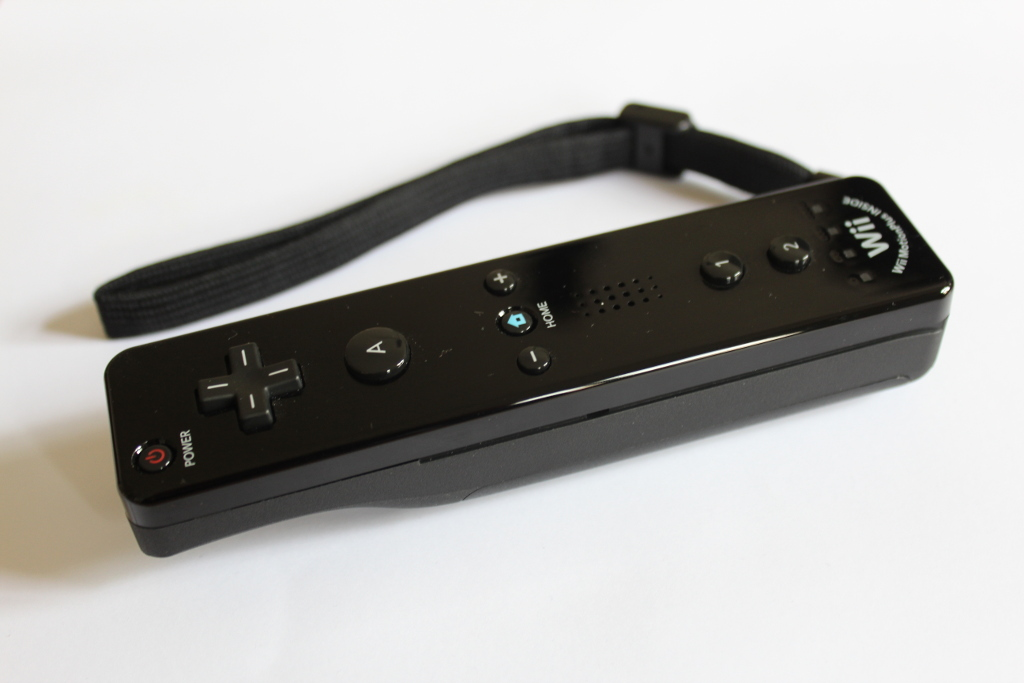
\includegraphics[width=0.5\textwidth]{wii-remote-plus-controller.JPG}
    \end{center}
    \caption{A black Wii Remote\texttrademark~Plus controller.}
    \label{fig:wii-remote}
\end{figure}
\subsection{Recording Setup} \label{recording_setup}
A Wii Remote\texttrademark~Plus controller is able to observe acceleration data in three axis via sensors. Those
acceleration data plus all button events on the controller can be send via
Bluetooth\footnote{https://www.bluetooth.com/} to another device. The other device was a computer that has executed the
recording software. Via a graphical user interface or shorten GUI the recording software instructed the experimentee to
perform gestures or physical activities. The experiment was a sequence of fullscreen slides that changed by performing a
gesture with the controller. Section \ref{data_recording_instructions} explains the specific sequence of slides. The
recording software observed all acceleration data and \textit{B} button events during the whole experiment and saved it
to a file. Marking the beginning and the end of a gesture was done with the \textit{B} button. The \textit{B}
button is on the bottom of the controller and triggered by the forefinger.

The recording software was implemented in Python\footnote{https://www.python.org/} and is available at
GitHub\footnote{https://github.com/GordonLesti/SlidingWindowFilter-experiment}. The main requirements for the recording
software are the open-source device driver for Nintendo Wii remotes,
xwiimote\footnote{https://github.com/dvdhrm/xwiimote} by David Herrmann and the language bindings for the xwiimote
package, xwiimote-bindings\footnote{https://github.com/dvdhrm/xwiimote-bindings} by Nicolas Adenis-Lamarre. The last
requirement was the main reason to implement the recording software in Python. For the GUI was choosen
TkInter\footnote{https://wiki.python.org/moin/TkInter}.

The first version of the recording software had the major problem to control the GUI and the
processing of the Bluetooth data in one loop with a linear flow. That caused a stagnation in the Bluetooth data queue
while loading new images in the GUI. This problem could be solved by two communicating threads and a preloading of the
images. Unfortunately, all existing records become unusable for the evaluation.

\subsubsection{File Format} \label{file_format}
Interesting for the evaluation of the experiment are the acceleration data in three axis and the \textit{B} button down
and up events to mark the beginning and the end of a gesture. This results in three different kinds of events, incoming
acceleration data, the \textit{B} button is pressed down and the \textit{B} button is released up. The controller is
sending the acceleration data with an average gap of five milliseconds. Every event has been marked with the time
in milliseconds that have passed since the starting of the experiment. The representing line in a recorded file for a
acceleration data event is starting with the time in milliseconds followed by the acceleration data of all three axis.
The acceleration data of a axis is transfered as integer value with the unit decimetre per second squared. A \textit{B}
button down event is represented by a line also starting with the time in milliseconds followed by the keyword
\textit{START} and a counter for the gesture. The \textit{B} button up event is the same with the keyword \textit{END}
instead of \textit{START}. An example excerpt of a recorded file can look like the following.

\medskip
\noindent
{\it Example excerpt of a recorded file}
\begin{verbatim}
3045 20 19 74
3050 16 12 70
3055 START 1
3055 14 13 88
3060 0 11 76
\end{verbatim}
\noindent
{\small Line 1, 2, 4 and 5 are representations of acceleration data and line 3 marks the beginning of the first gesture
triggered by a \textit{B} button down event.}

\medskip

The recorded files are evaluated in section \ref{evaluation}. All
recorded files used in the evaluation are available on
GitHub\footnote{https://github.com/GordonLesti/SlidingWindowFilter-evaluator/tree/v1.0.1/src/main/resources}.


\subsection{Data Recording Instructions} \label{data_recording_instructions}
The recording instructions of the experiment are containing 16 slides plus one slide for the welcoming and two slides
for thanking the experimentee and saying goodbye. The slides change after every performed gesture. A gesture can
be performed by pressing the \textit{B} button, moving the controller and releasing the \textit{B} button after the
gesture. As mentioned in section \ref{experiment}, the experiment consists of two parts, the recording of 8 training
gestures and the repetition of those gestures mixed with physical activities. All slides of the experiment are shown in
figure~\ref{fig:slides}.

\begin{figure}
    \begin{center}
        \resizebox {\textwidth} {!} {
            \begin{tabular}{cccc}
                \frame{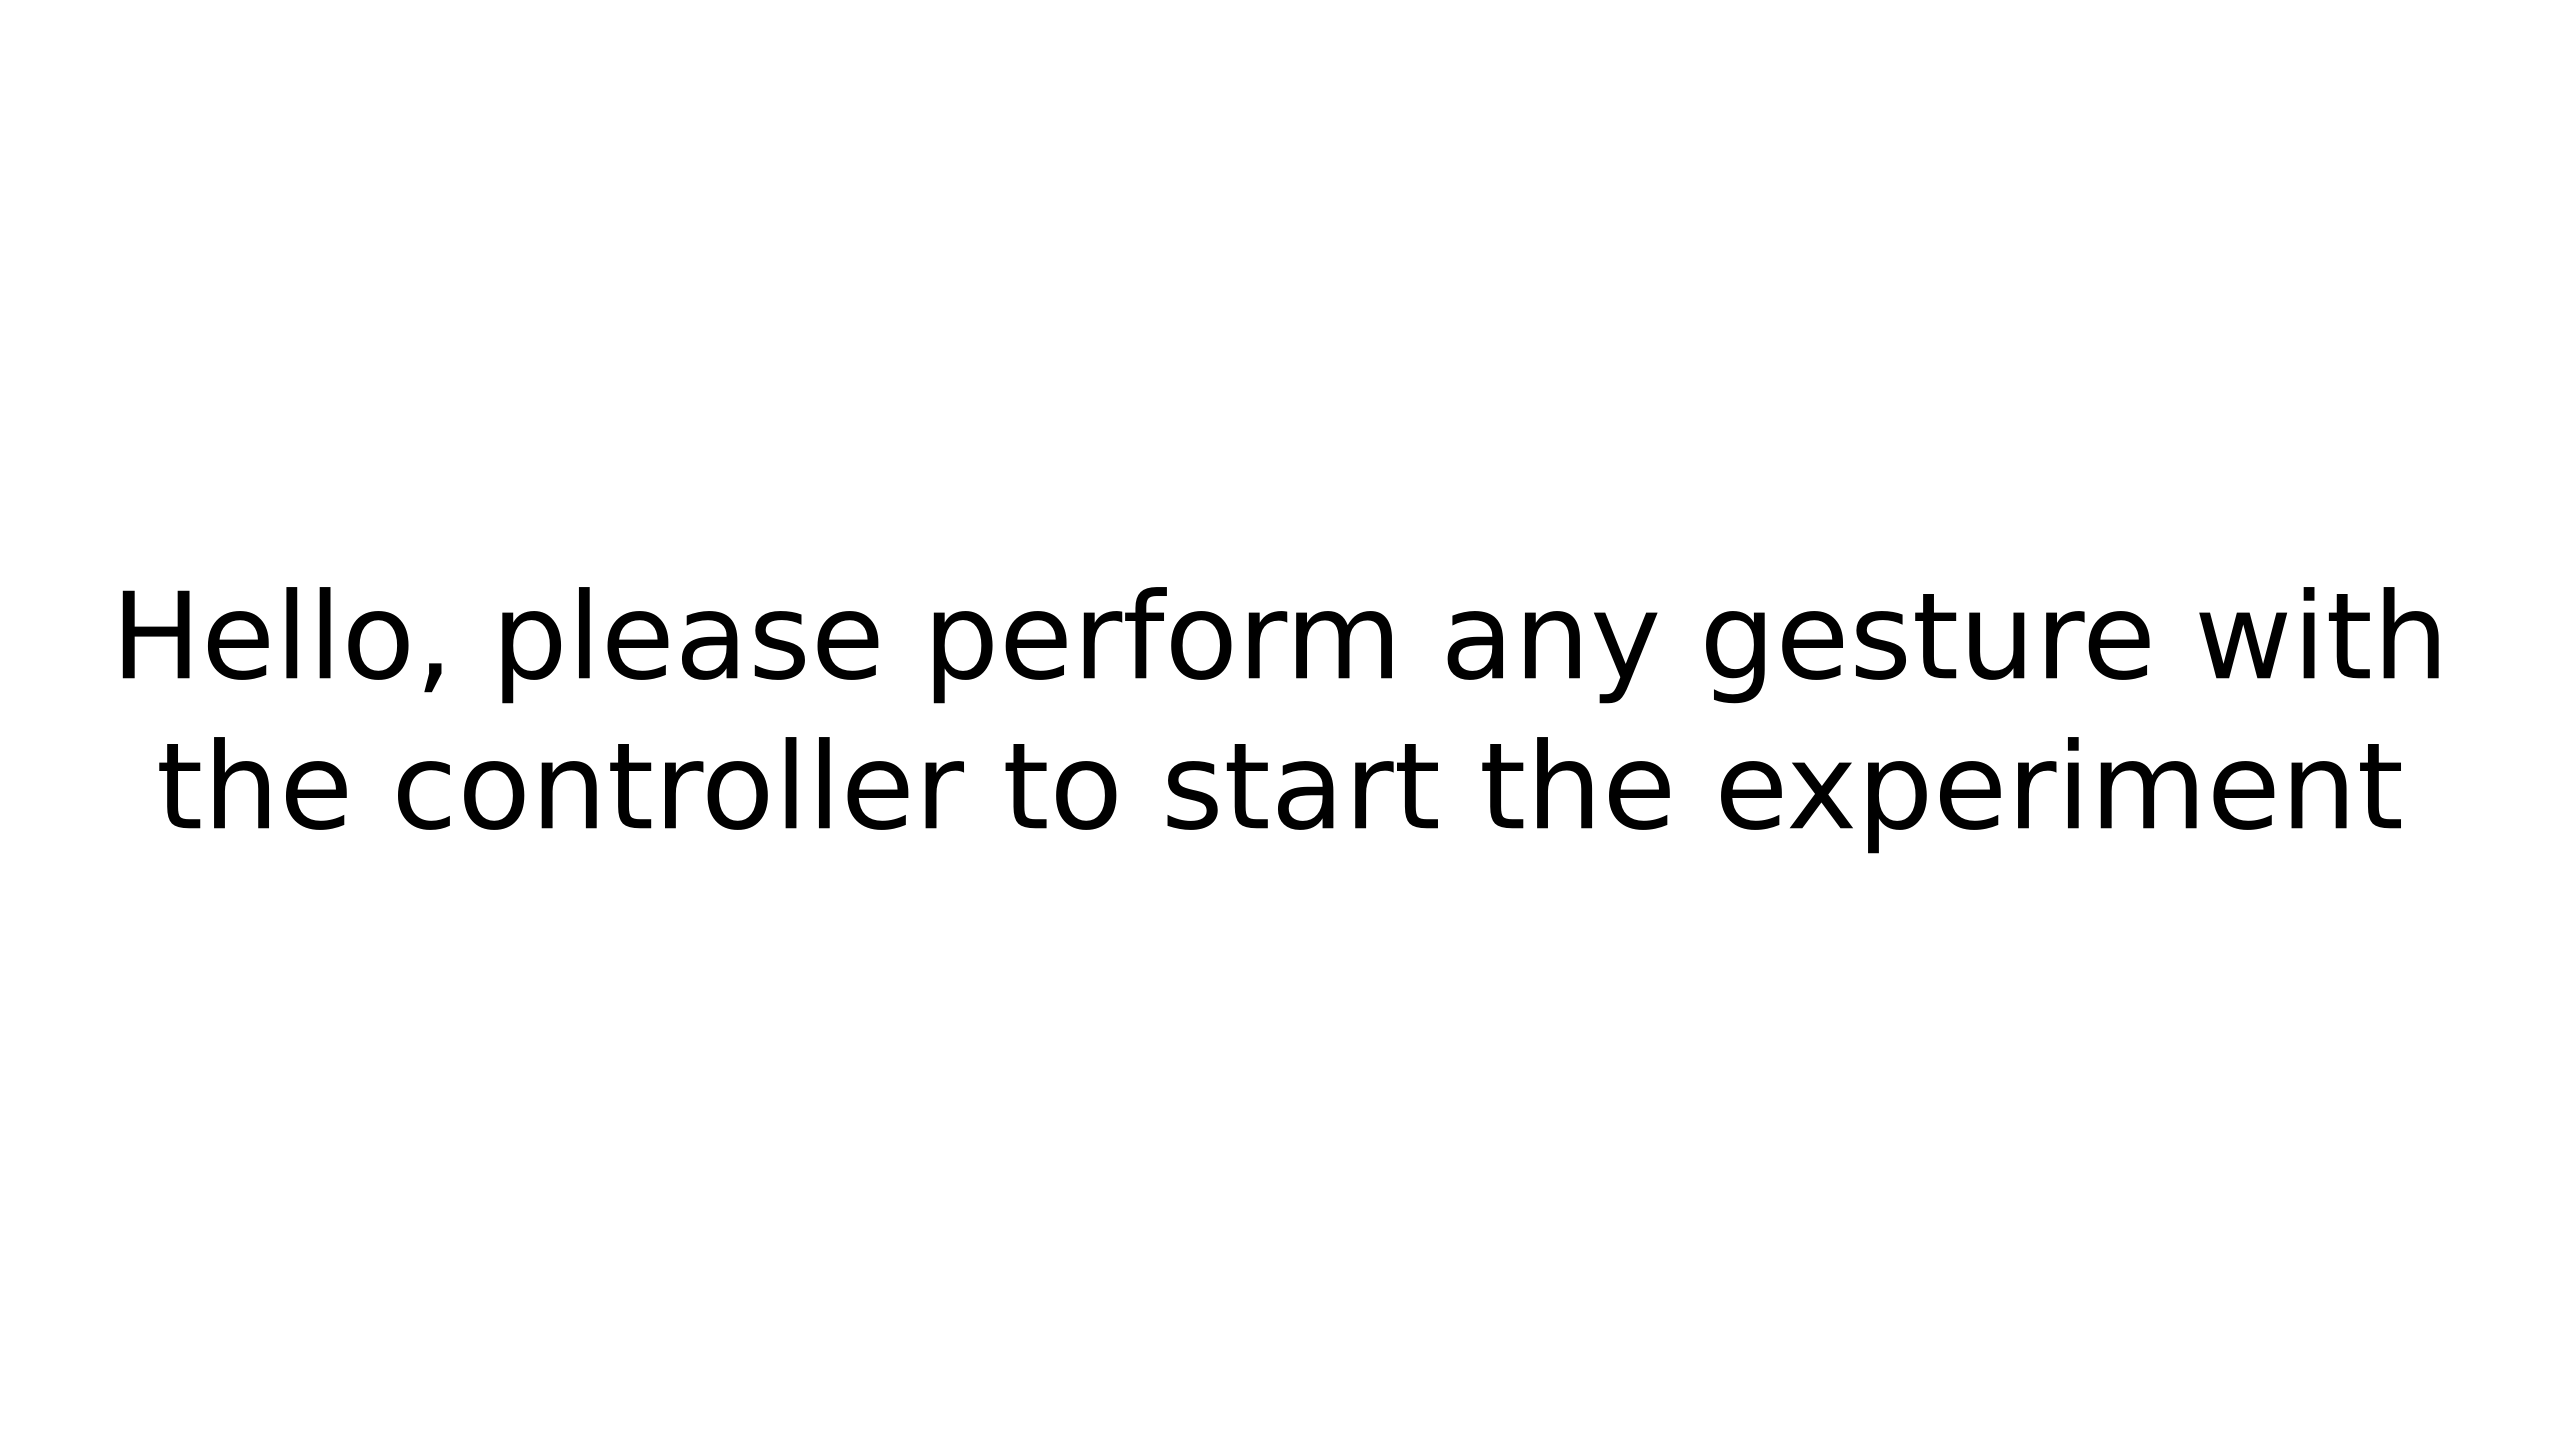
\includegraphics[width=0.25\textwidth]{1.png}} &
                \frame{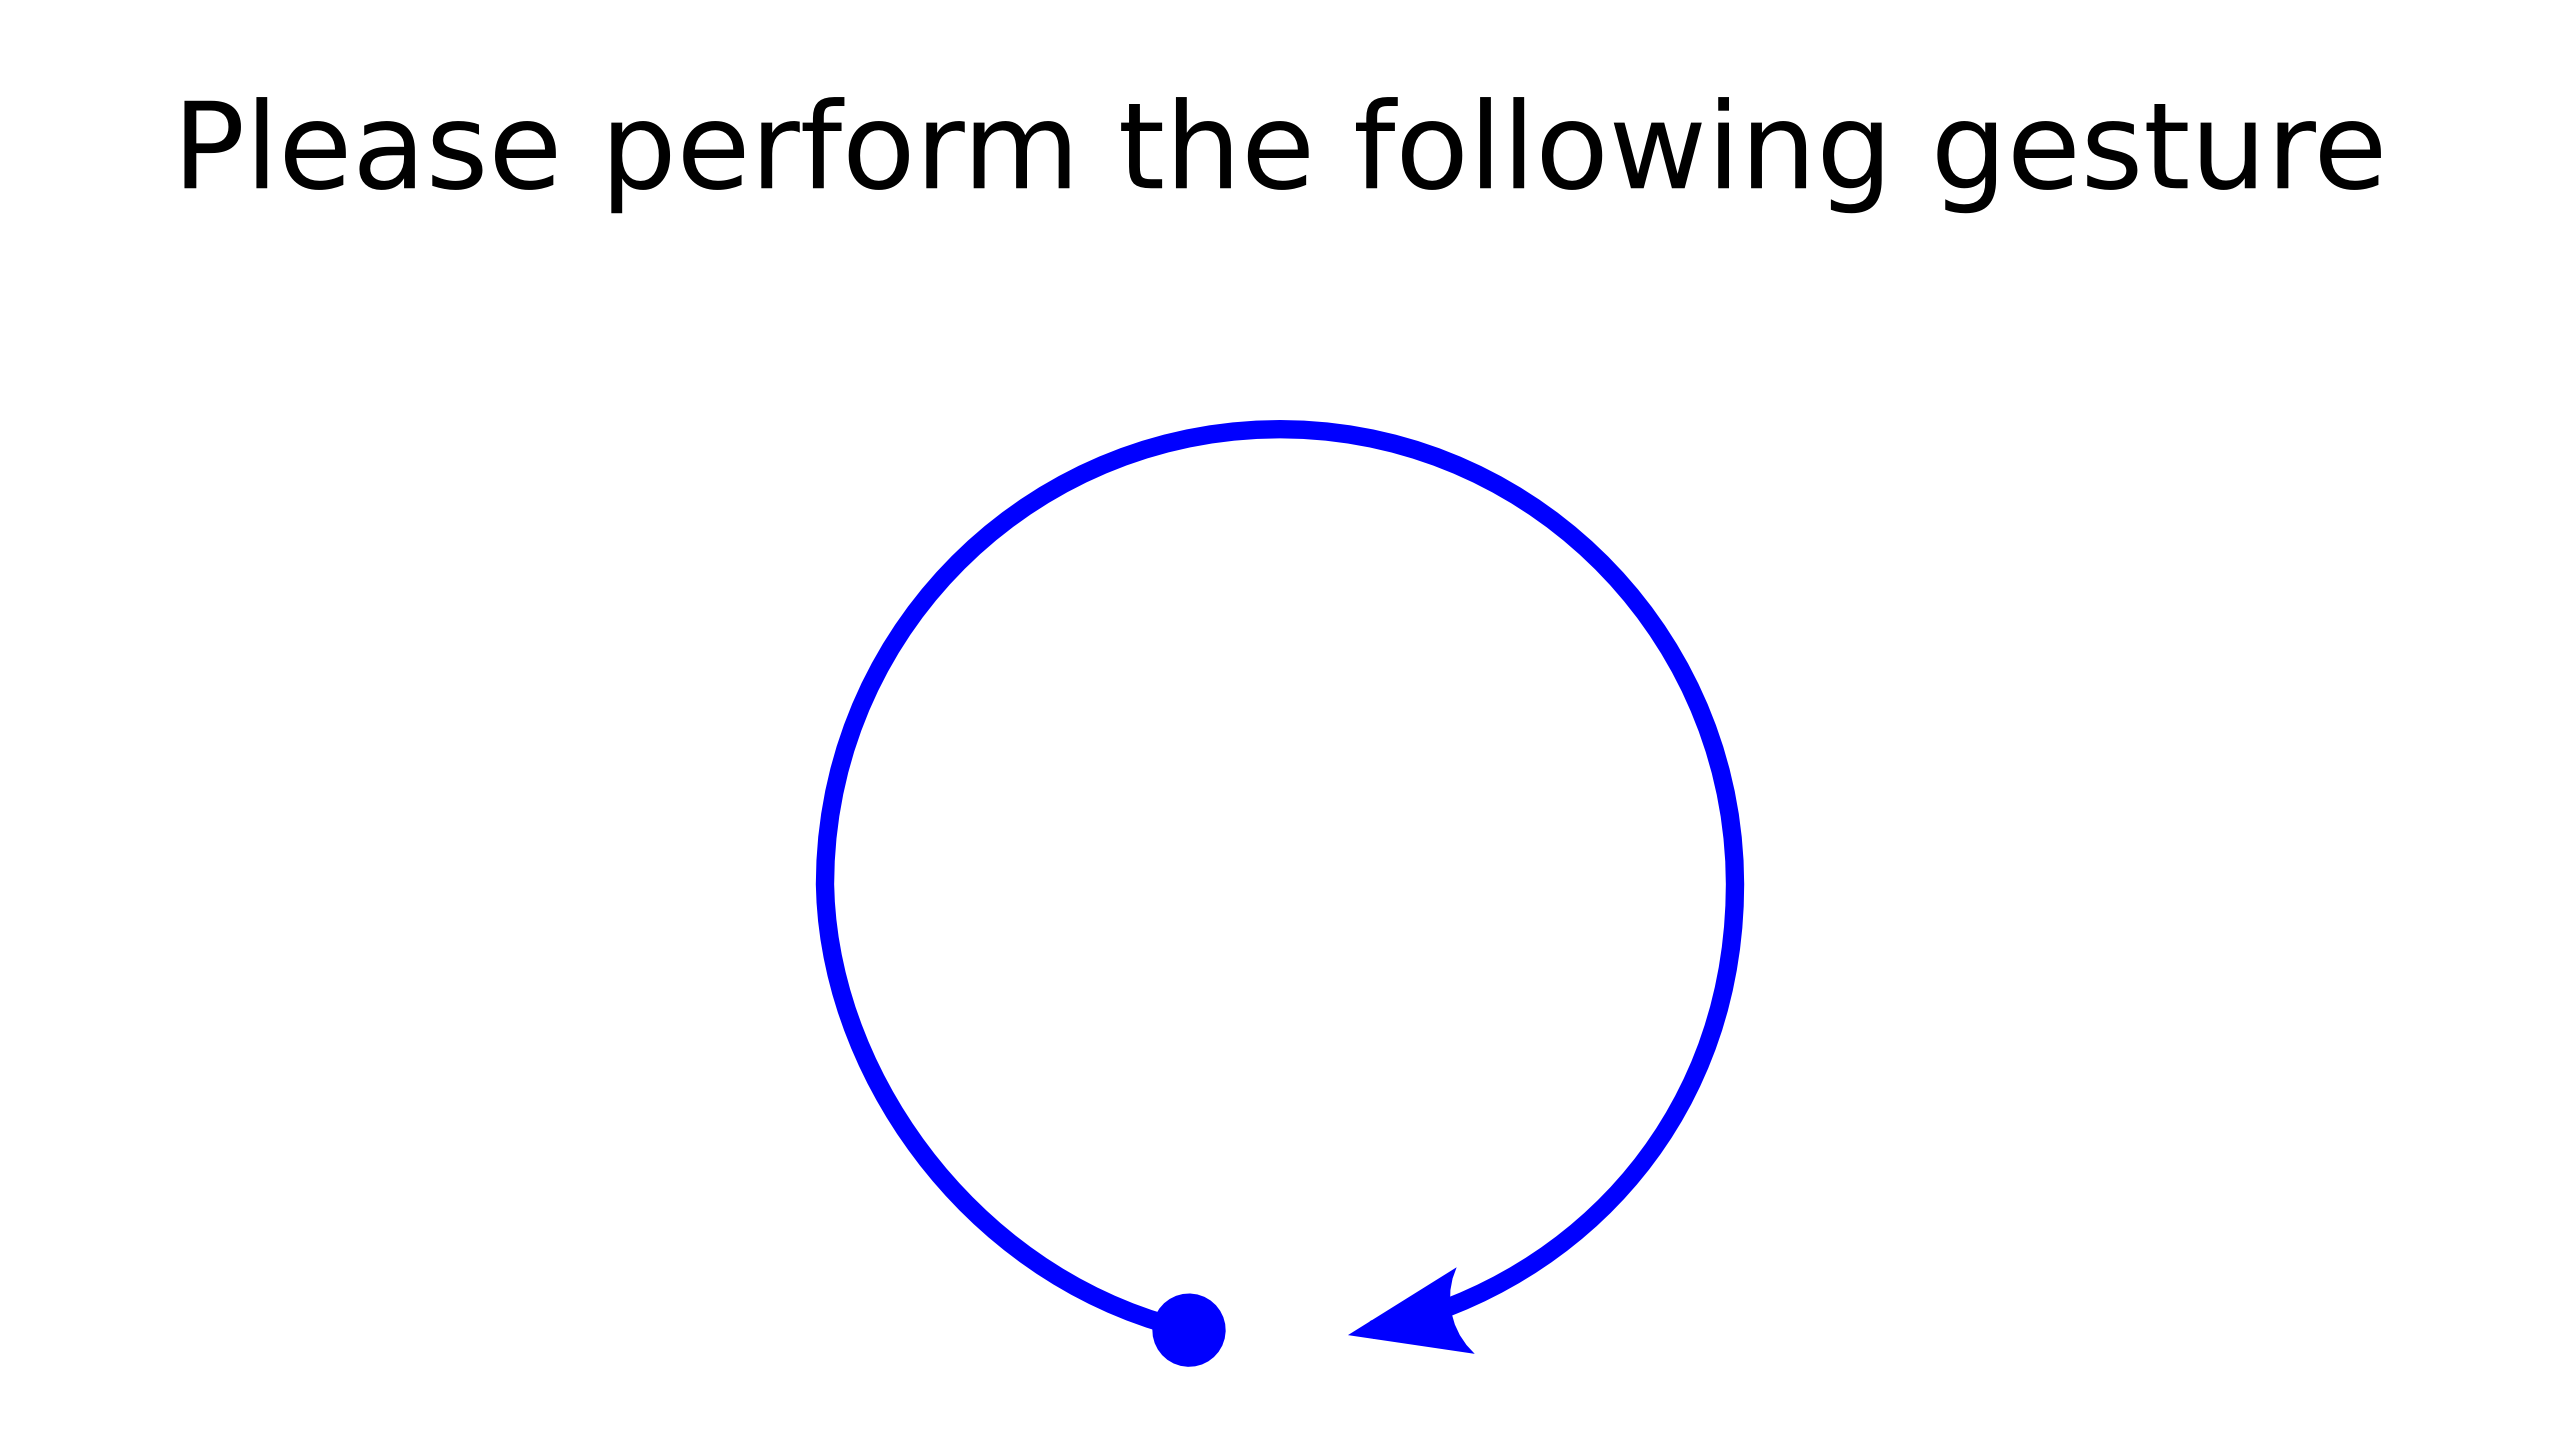
\includegraphics[width=0.25\textwidth]{2.png}} &
                \frame{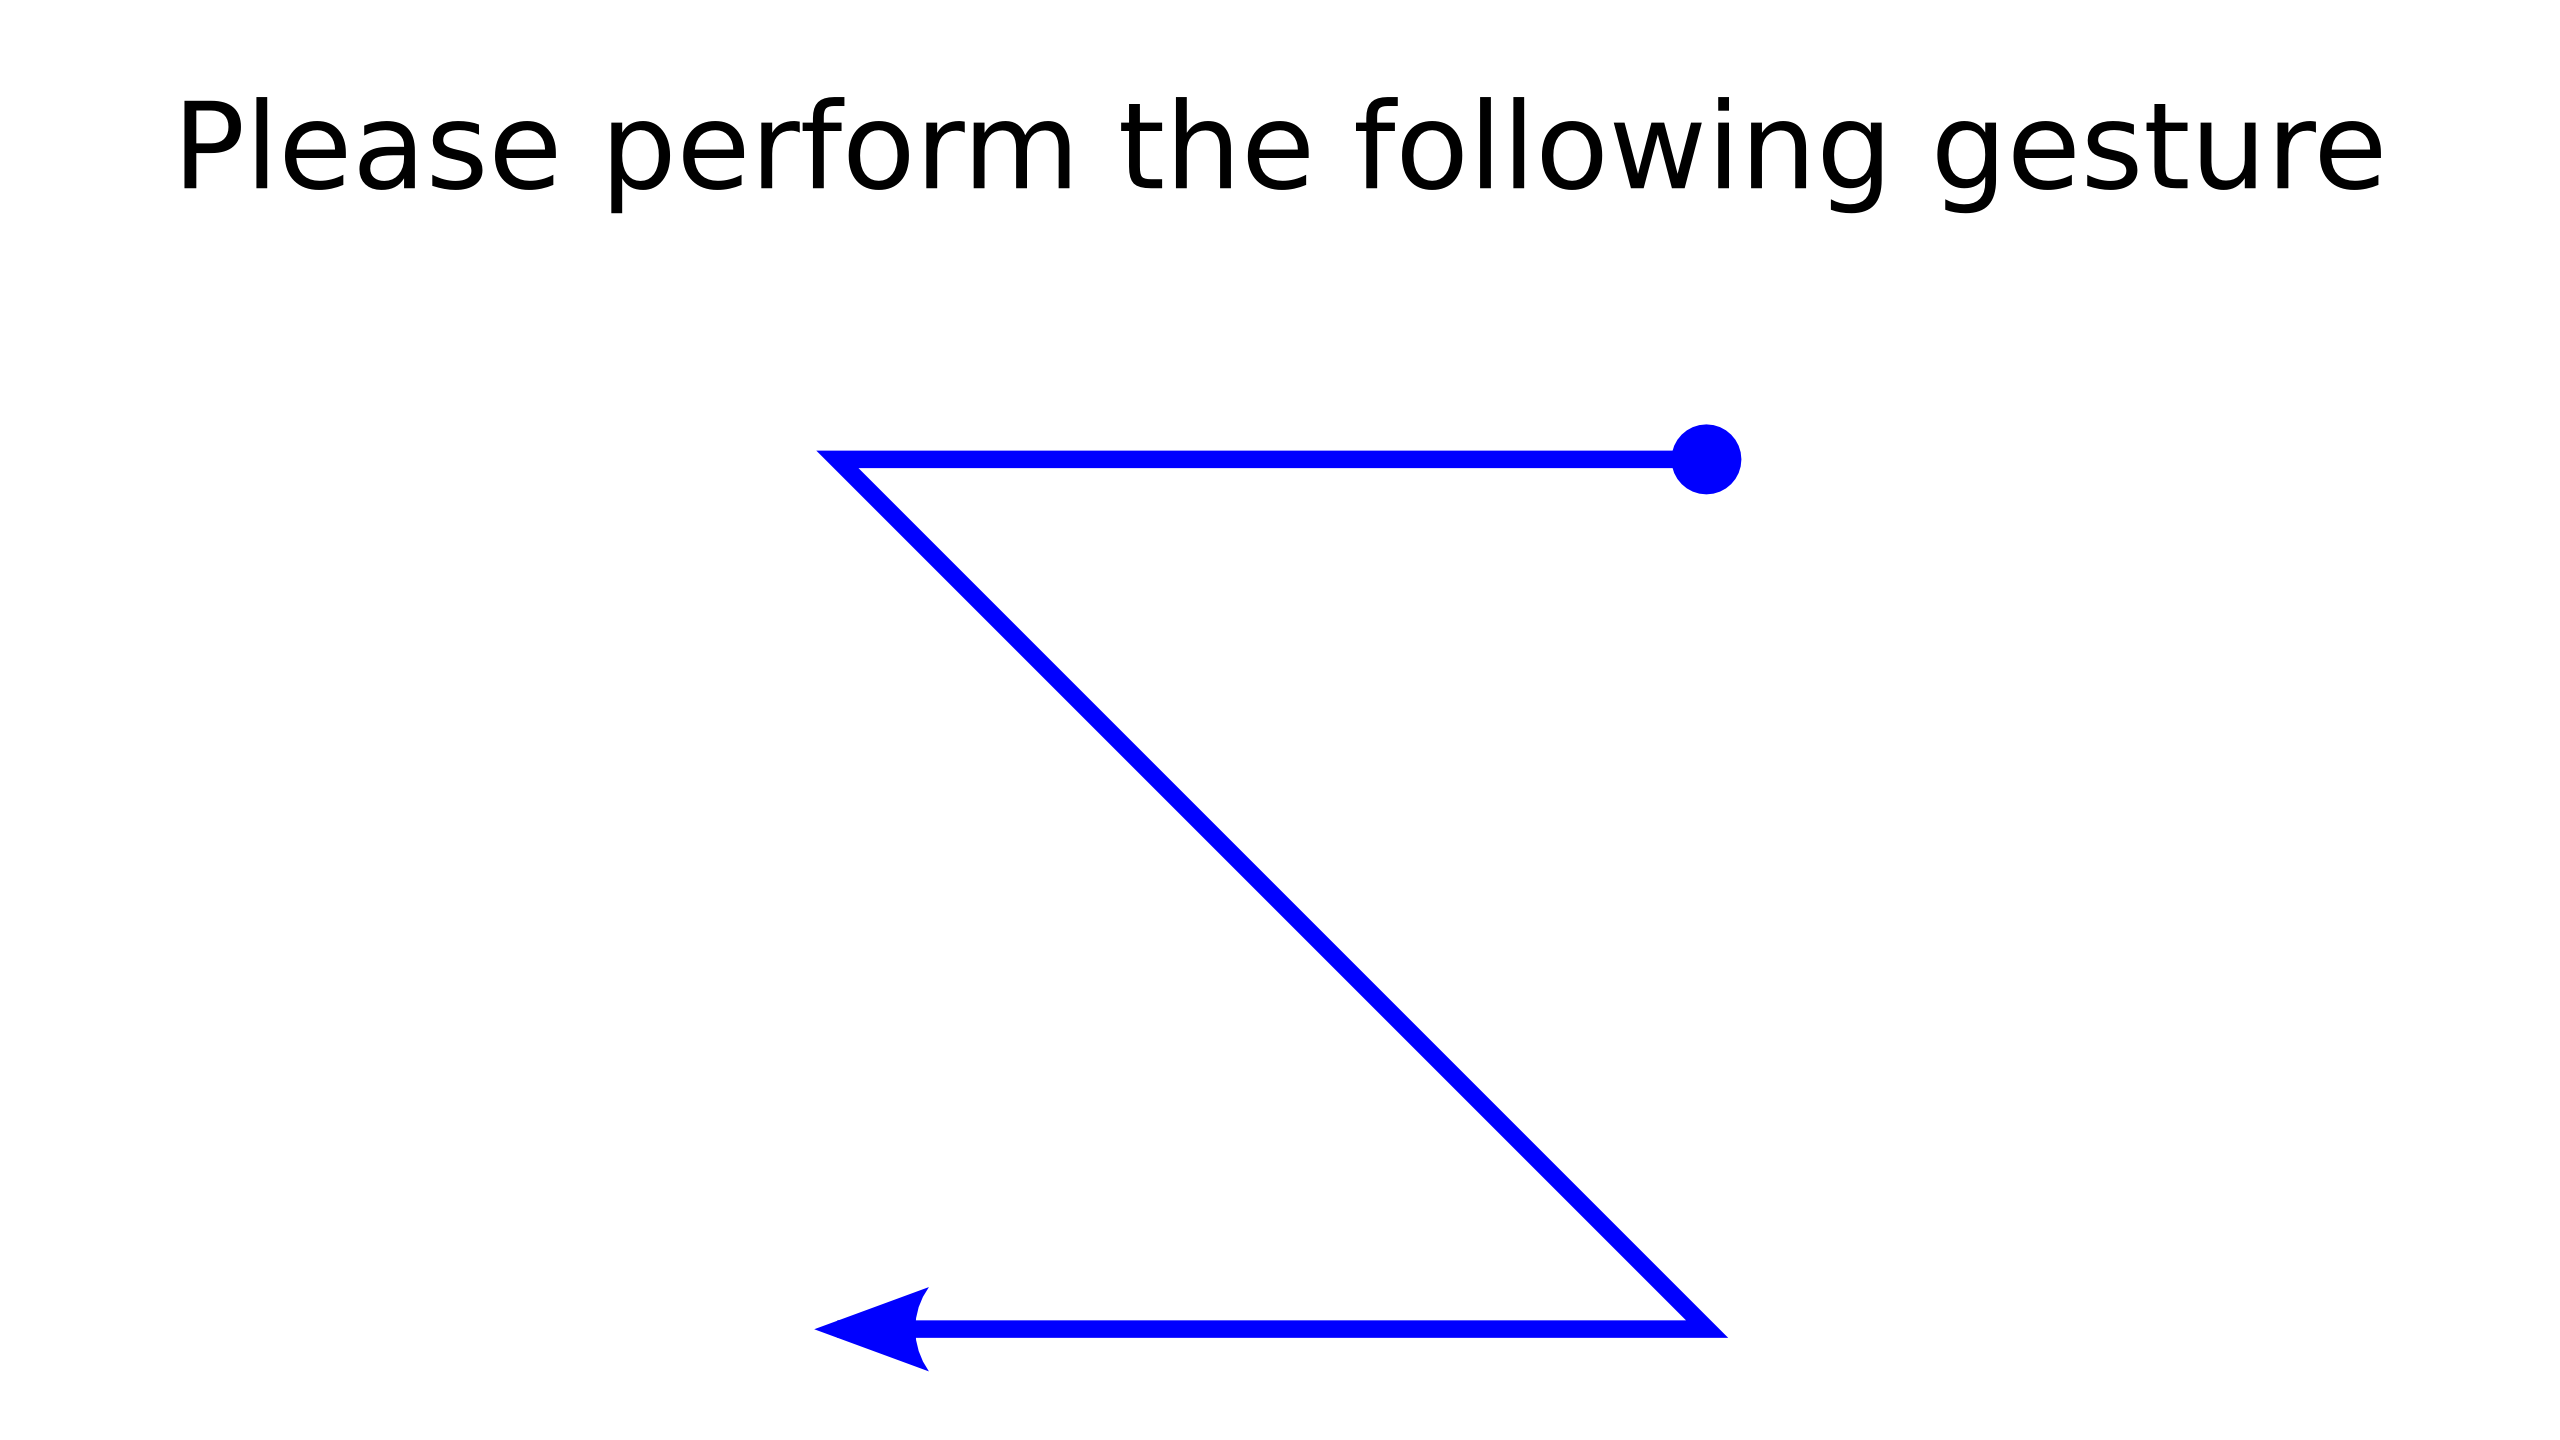
\includegraphics[width=0.25\textwidth]{3.png}} &
                \frame{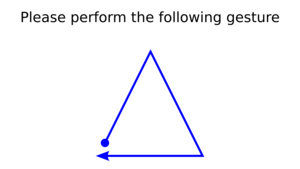
\includegraphics[width=0.25\textwidth]{4.png}} \\
                (a) \vspace{0.5ex} & (b) \vspace{0.5ex} & (c) \vspace{0.5ex} & (d) \vspace{0.5ex} \\
                \frame{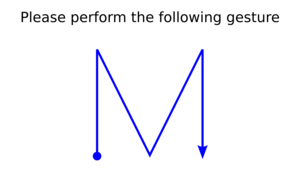
\includegraphics[width=0.25\textwidth]{5.png}} &
                \frame{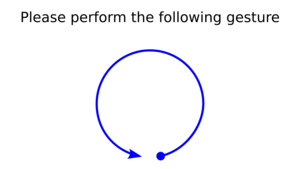
\includegraphics[width=0.25\textwidth]{6.png}} &
                \frame{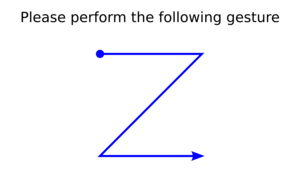
\includegraphics[width=0.25\textwidth]{7.png}} &
                \frame{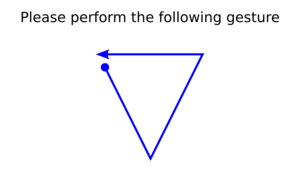
\includegraphics[width=0.25\textwidth]{8.png}} \\
                (e) \vspace{0.5ex} & (f) \vspace{0.5ex} & (g) \vspace{0.5ex} & (h) \vspace{0.5ex} \\
                \frame{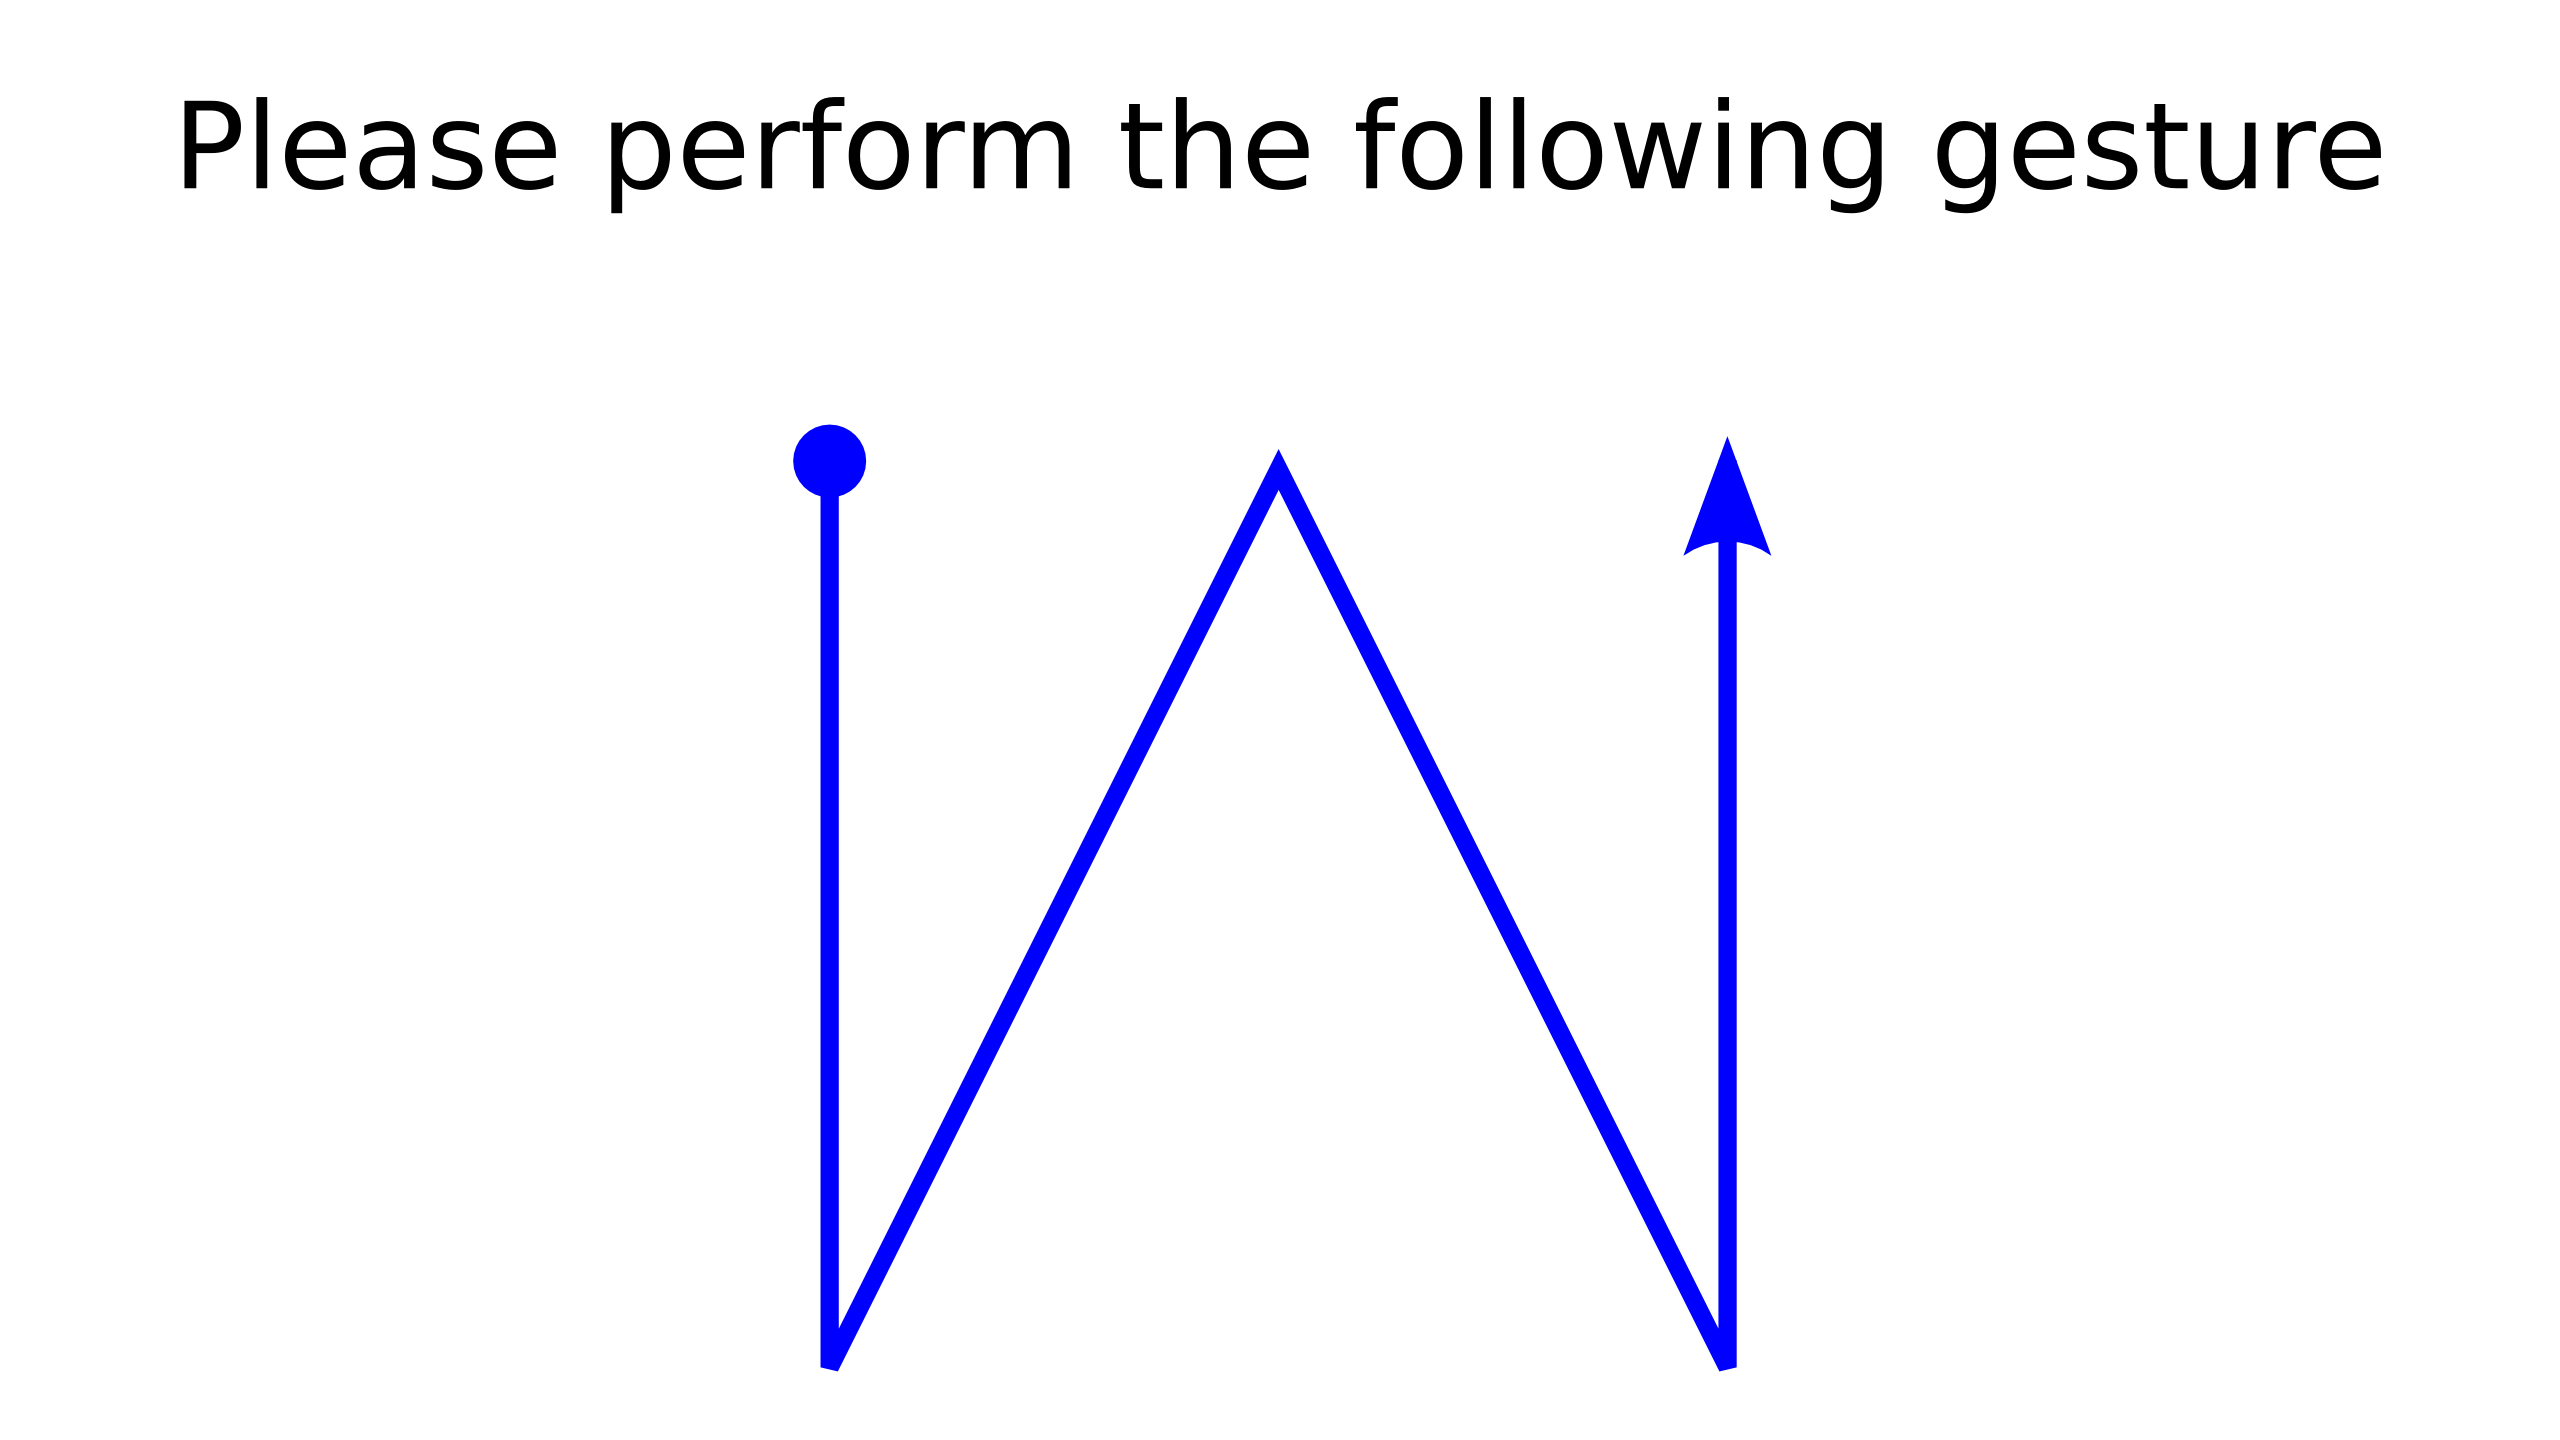
\includegraphics[width=0.25\textwidth]{9.png}} &
                \frame{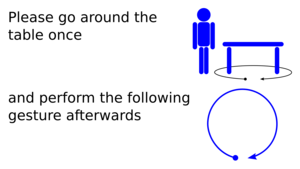
\includegraphics[width=0.25\textwidth]{10.png}} &
                \frame{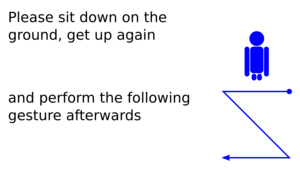
\includegraphics[width=0.25\textwidth]{11.png}} &
                \frame{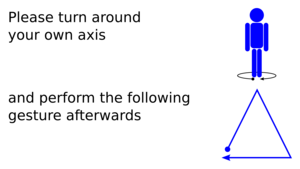
\includegraphics[width=0.25\textwidth]{12.png}} \\
                (i) \vspace{0.5ex} & (j) \vspace{0.5ex} & (k) \vspace{0.5ex} & (l) \vspace{0.5ex} \\
                \frame{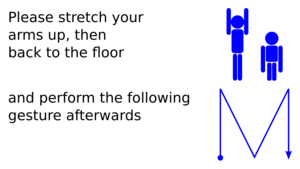
\includegraphics[width=0.25\textwidth]{13.png}} &
                \frame{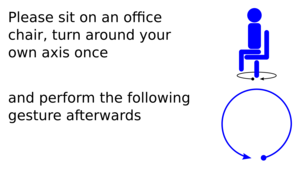
\includegraphics[width=0.25\textwidth]{14.png}} &
                \frame{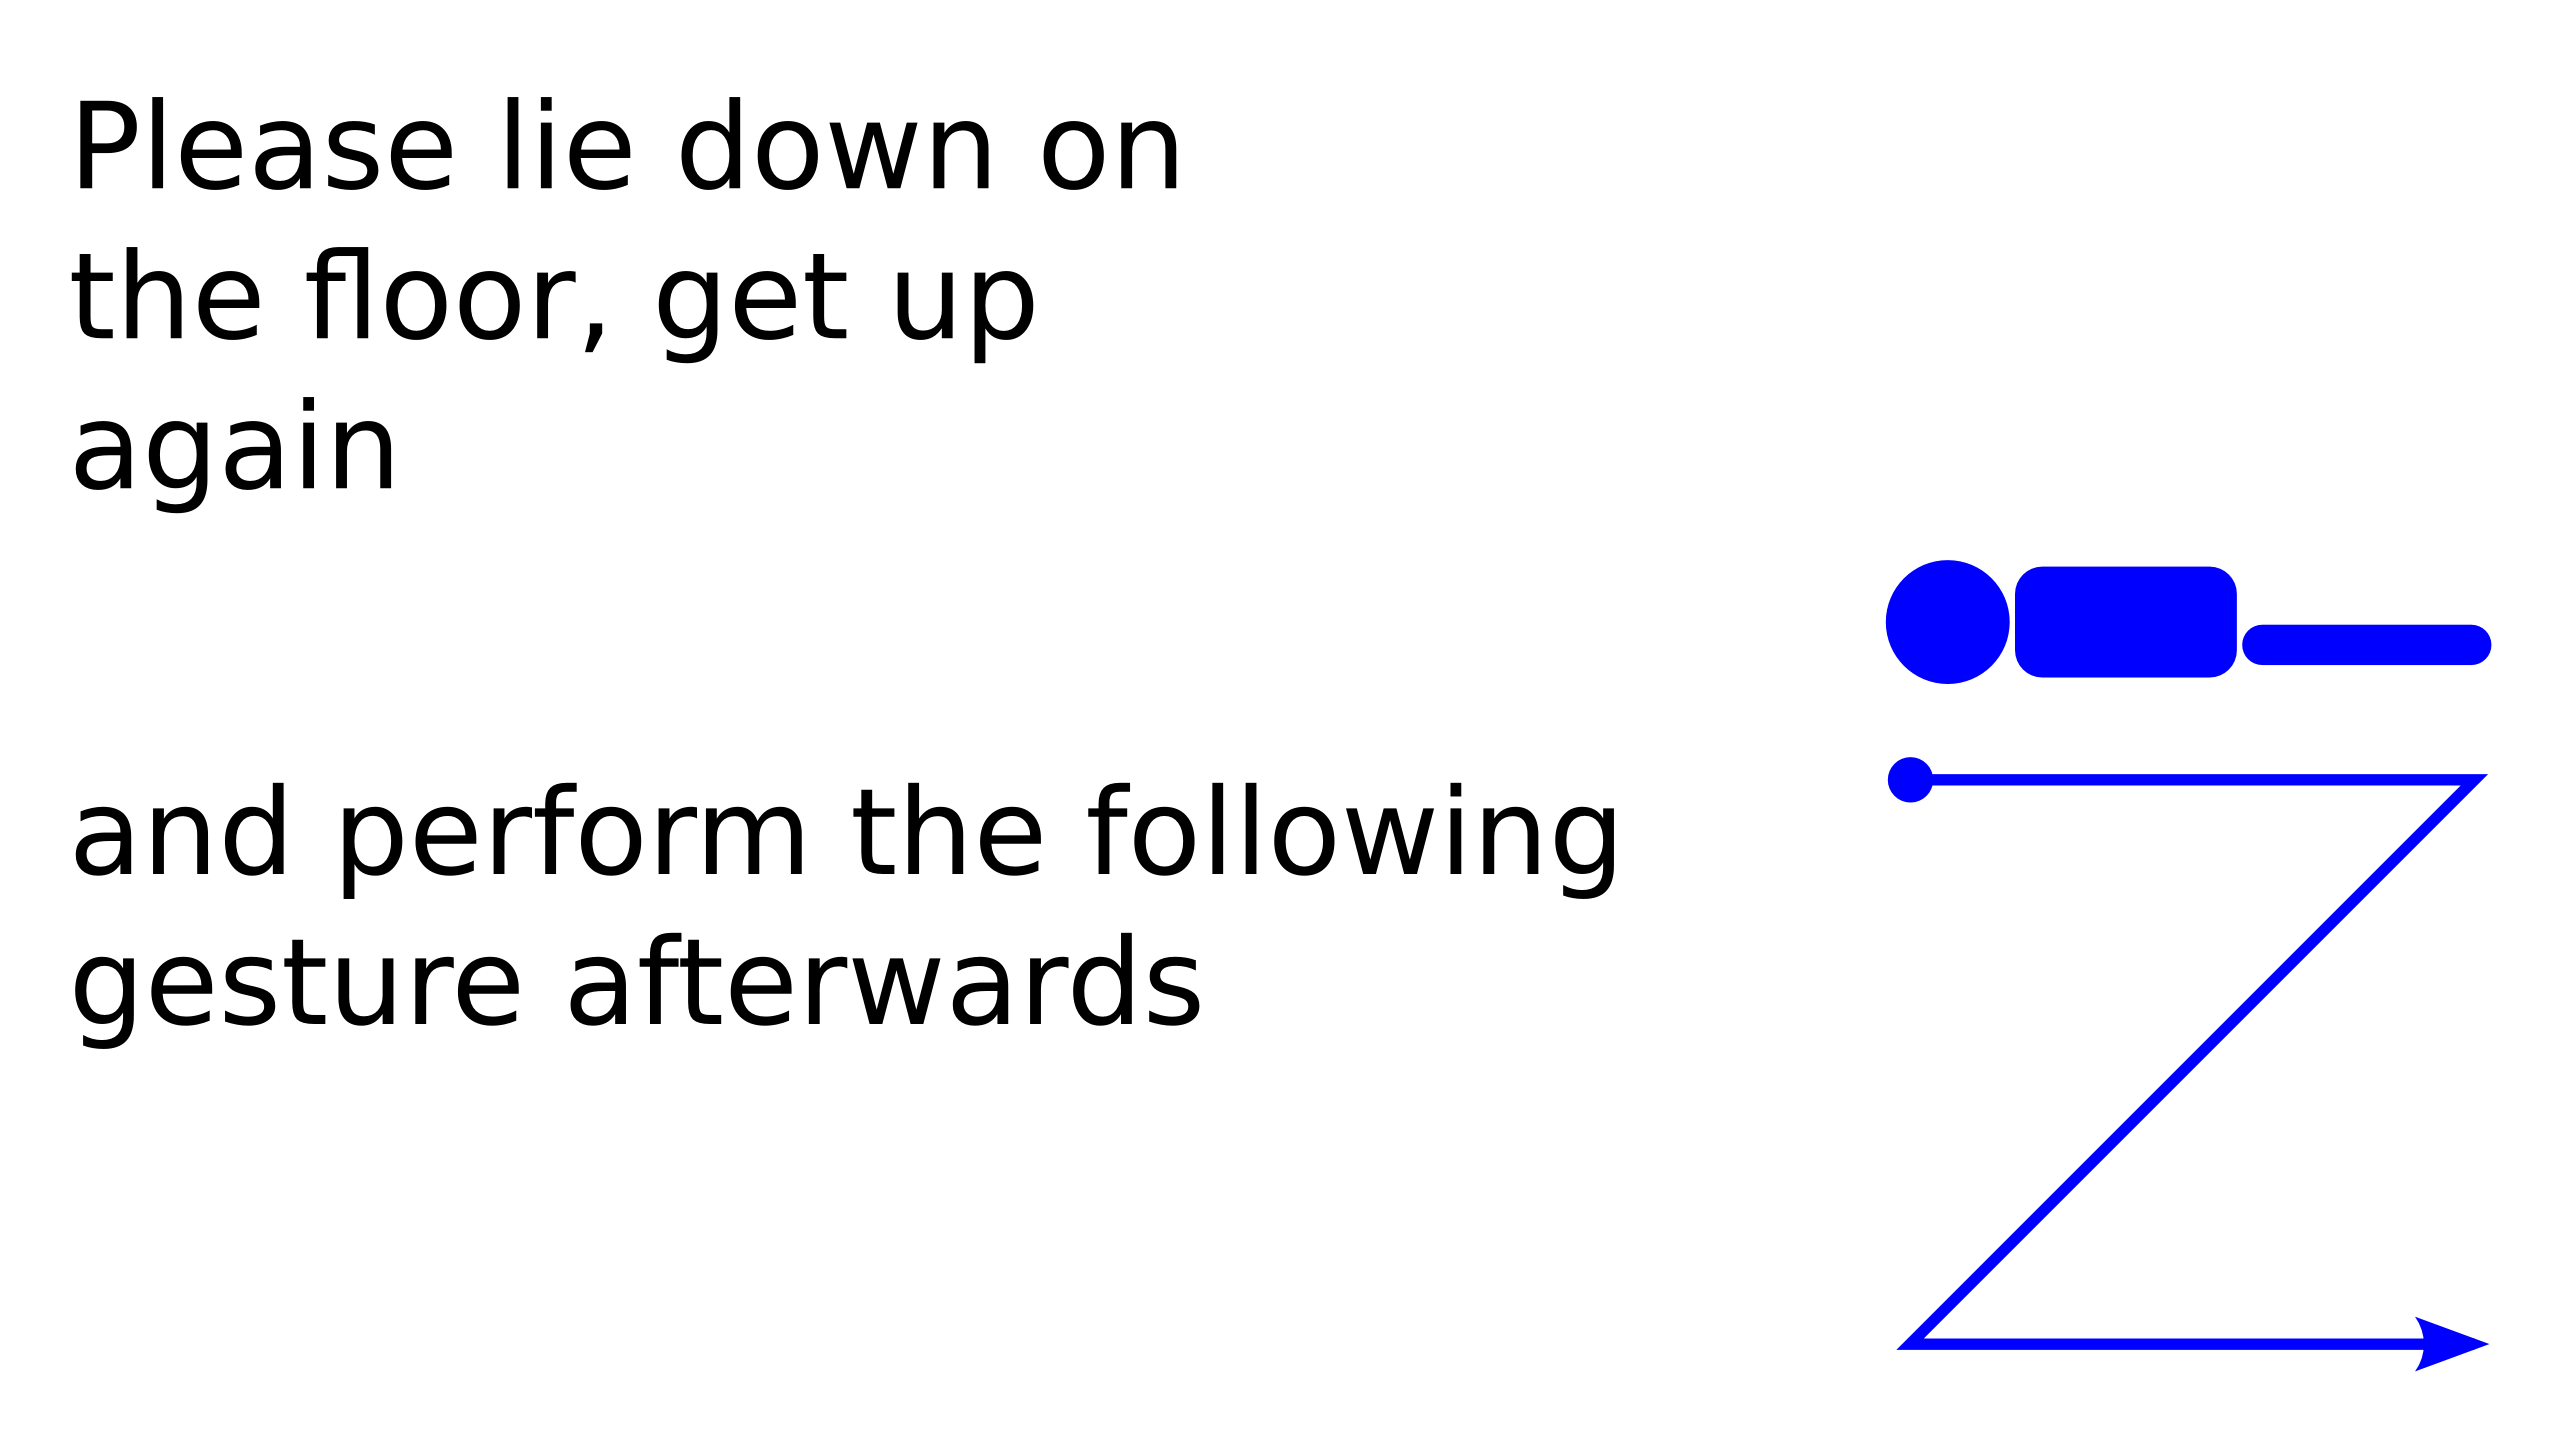
\includegraphics[width=0.25\textwidth]{15.png}} &
                \frame{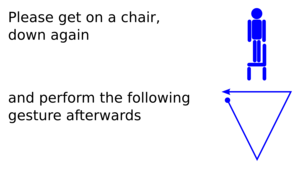
\includegraphics[width=0.25\textwidth]{16.png}} \\
                (m) \vspace{0.5ex} & (n) \vspace{0.5ex} & (o) \vspace{0.5ex} & (p) \vspace{0.5ex} \\
                \frame{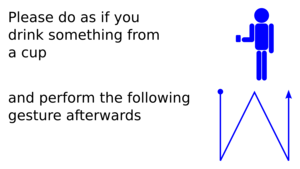
\includegraphics[width=0.25\textwidth]{17.png}} &
                \frame{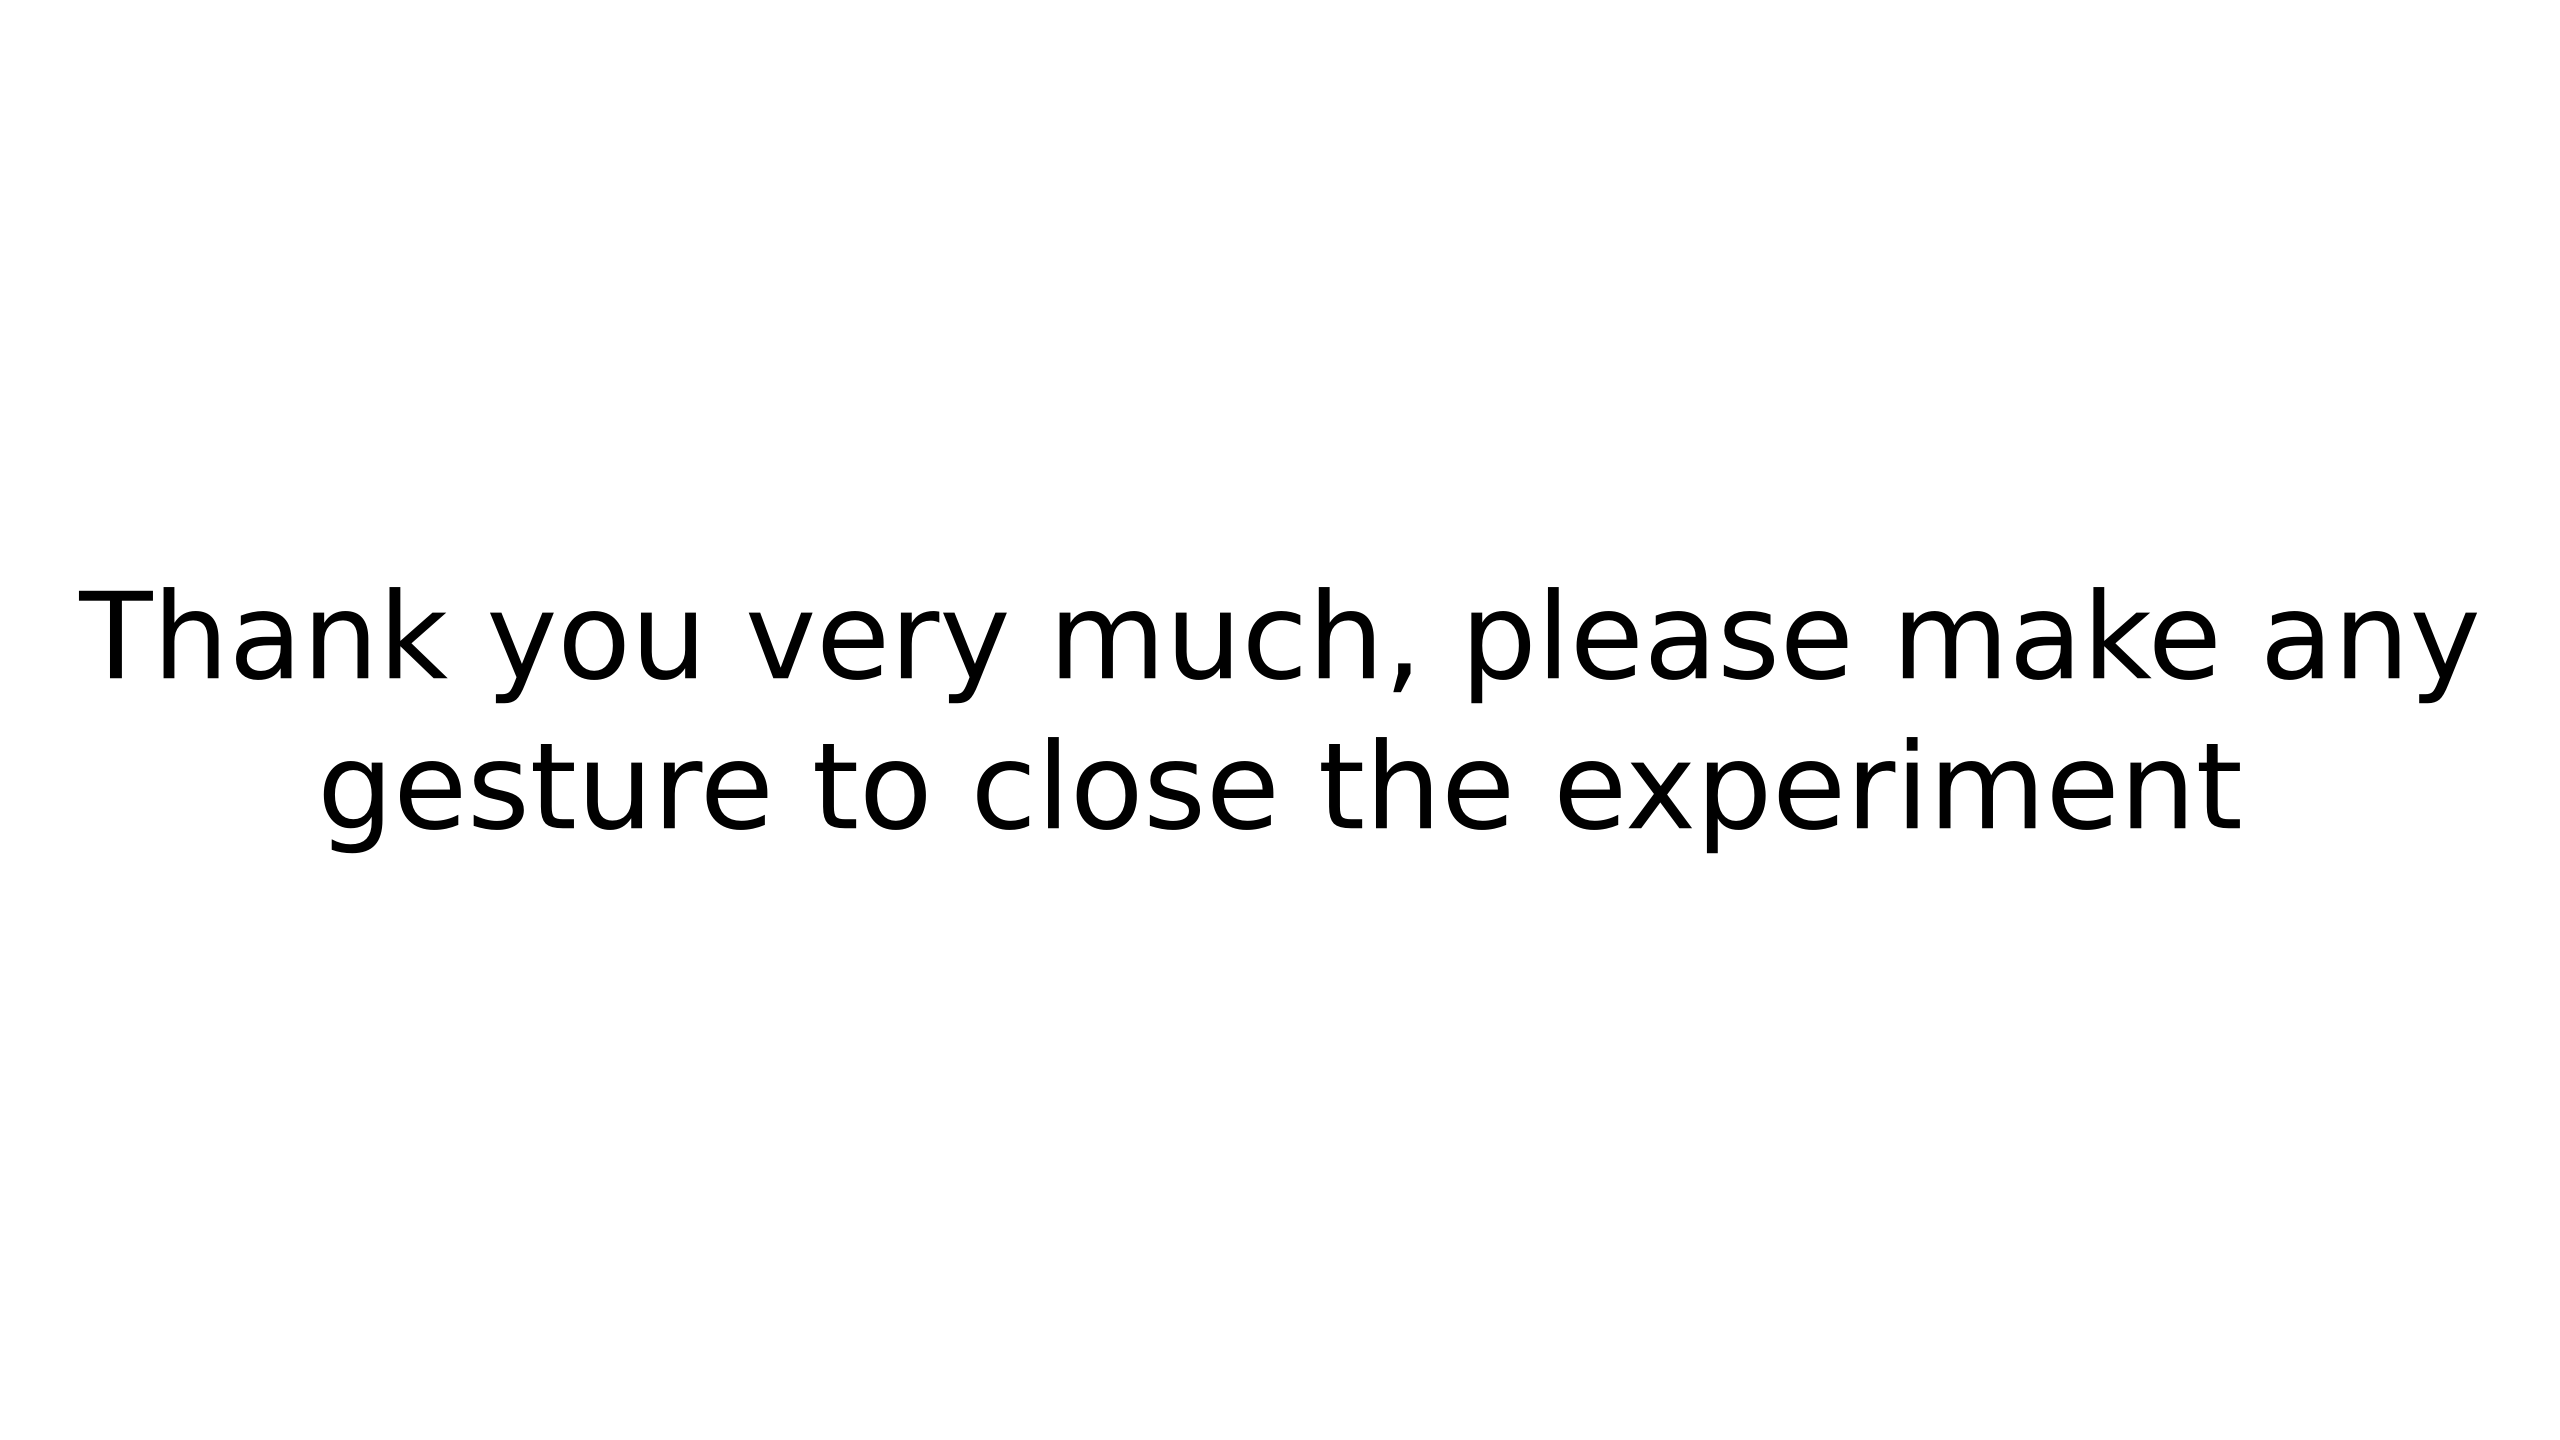
\includegraphics[width=0.25\textwidth]{18.png}} &
                \frame{
\includegraphics[width=0.25\textwidth]{19.png}} & \\
                (q) & (r) & (s) & \\
            \end{tabular}
        }
    \end{center}
    \caption{The slides that are guiding the experimentees.}
    \label{fig:slides}
\end{figure}

Slide (a) of figure \ref{fig:slides} has the task to welcome the experimentee and is later used in experimental protocol
to mark the start of the recording. The slides (b) to (i) of figure \ref{fig:slides} have the task to create training
data for 1NN-DTW. Physical activities mixed with the same gestures from (b) to (i) are on the slides (j) to (q) of
figure \ref{fig:slides}. The recorded acceleration data from slide (j) to (q) of figure \ref{fig:slides} will simulate
the time series stream in section \ref{experimental_protocol}. Slide (r) of figure \ref{fig:slides} and the last
insignificant gesture have the task to prevent an abrupt ending of the record. The last slide (s) of figure
\ref{fig:slides} closes the recording applciation.

\subsubsection{Gesture Notation} \label{gesture_notation}
The \textit{clockwise circle} gesture of slide (b) and (j) in figure \ref{fig:slides} is abbreviated with $GesA$, the
\textit{flipped Z} gesture on slide (c) and (k) of figure \ref{fig:slides} is abbreviated with $GesB$ and so on until
the \textit{W} gesture of slide (i) and (q) in figure \ref{fig:slides} shortend with $GesH$.

As the experiment was executed by different experimentees a instance of gesture $GesC$ performed by the fourth
experimentee on slide (d) of figure \ref{fig:slides} will be abbreviated as $exp_{4}.GesC_{1}$. The same gesture by the
same experimentee on slide (l) of figure \ref{fig:slides} will be abbreviated as $exp_{4}.GesC_{2}$.


\subsection{Experimental Protocol} \label{experimental_protocol}
The software to evaluate the recorded data has been written in Java\footnote{https://www.java.com/} and is available on
GitHub\footnote{https://github.com/GordonLesti/SlidingWindowFilter-evaluator}. The requirements are
OpenJDK\footnote{http://openjdk.java.net/} 8 to run the code and Gradle\footnote{https://gradle.org/} 3.3 to test the
code and build the executable binaries.

\subsubsection{Quantization} \label{quantization}
All recorded data were quantized before evaluation. The authors of \cite{liu2009uwave} have two reasons for that,
the length of the time series were reduced for DTW in order to improve computation efficiency and the recorded time
series was transformed with a stable time gab between the data points. The quantization process of
\cite{liu2009uwave} is used in this bachelor thesis. The quantization process of a recorded gesture is
illustrated by figure \ref{fig:quantization}.

\paragraph{Compressing} The recorded acceleration data were compressed to an average value for a window size of 50
ms and a step length of 30 ms.

\paragraph{Conversion} The compressed records are converted into 33 different levels that are summarized in
table \ref{table:conversion}.

\begin{table}
    \begin{center}
        \begin{tabularx}{\textwidth}{XX}
            \hline
            \textbf{Acceleration data ($a$) in $\frac{dm}{s^2}$} & \qquad \textbf{Converted value}\\
            \hline
            $a > 200$ & \qquad 16\\
            $100 < a < 200$ & \qquad 11 to 15 (five levels linearly)\\
            $0 < a < 100$ & \qquad 1 to 10 (ten levels linearly)\\
            $a = 0$ & \qquad 0\\
            $-100 < a < 0$ & \qquad -1 to - 10 (ten levels linearly)\\
            $-200 < a < -100$ & \qquad -11 to - 15 (five levels linearly)\\
            $a < -200$ & \qquad -16\\
            \hline
        \end{tabularx}
    \end{center}
    \caption{Table shows the conversion rules of the recorded acceleration data. In contrast to \cite{liu2009uwave} are
    $100\frac{dm}{s^2}$ the steps threshold and not $1g$.}
	\label{table:conversion}
\end{table}

\begin{figure}
    \begin{center}
        \resizebox {\textwidth} {!} {
            \begin{tabular}{ccc}
                \resizebox {!} {\height} {
                    \begin{tikzpicture}
                        \begin{axis}[
                            xmin=1,
                            xmax=295,
                            xlabel=time,
                            ylabel=acceleration in $\frac{dm}{s^2}$]
                            \addplot[blue, ultra thick, mark=none] table[x=t, y=x] {experiment/experimental_protocol/quantization/raw.dat};
                            \addplot[red, ultra thick, mark=none] table[x=t, y=y] {experiment/experimental_protocol/quantization/raw.dat};
                            \addplot[green, ultra thick, mark=none] table[x=t, y=z] {experiment/experimental_protocol/quantization/raw.dat};
                        \end{axis}
                    \end{tikzpicture}
                } &
                \resizebox {!} {\height} {
                    \begin{tikzpicture}
                        \pgfplotsset{every axis legend/.append style={
                    		at={(0.5,1.03)},
                    		anchor=south}}
                        \begin{axis}[
                            xmin=1,
                            xmax=52,
                            xlabel=time,
                            ylabel=acceleration in $\frac{dm}{s^2}$,
                            legend columns=4]
                            \addplot[blue, ultra thick, mark=none] table[x=t, y=x] {experiment/experimental_protocol/quantization/compressed.dat};
                            \addlegendentry{x-axis}
                            \addplot[red, ultra thick, mark=none] table[x=t, y=y] {experiment/experimental_protocol/quantization/compressed.dat};
                            \addlegendentry{y-axis}
                            \addplot[green, ultra thick, mark=none] table[x=t, y=z] {experiment/experimental_protocol/quantization/compressed.dat};
                            \addlegendentry{z-axis}
                        \end{axis}
                    \end{tikzpicture}
                } &
                \resizebox {!} {\height} {
                    \begin{tikzpicture}
                        \begin{axis}[
                            xmin=1,
                            xmax=52,
                            xlabel=time,
                            ylabel=converted acceleration]
                            \addplot[blue, ultra thick, mark=none] table[x=t, y=x] {experiment/experimental_protocol/quantization/converted.dat};
                            \addplot[red, ultra thick, mark=none] table[x=t, y=y] {experiment/experimental_protocol/quantization/converted.dat};
                            \addplot[green, ultra thick, mark=none] table[x=t, y=z] {experiment/experimental_protocol/quantization/converted.dat};
                        \end{axis}
                    \end{tikzpicture}
                }
            \end{tabular}
        }
    \end{center}
    \caption{The left plot shows the raw recorded gesture for all three axis. On the middle plot are the compressed
    acceleration data of the gesture. The right plot shows the converted and compressed gesture.}
    \label{fig:quantization}
\end{figure}

\subsubsection{Labeled Generic Time Series Model} \label{labeled_generic_time_series_model}
A generic time series model was created for the evaluating software. A generic time series over the domain set
$\mathbb{U}$ will be a linked list of data points. Those data points are containing a generic data object and an
optional label. The generic object has to be an element of the domain set $\mathbb{U}$. In the case of the carried out
experiment a data point contains the acceleration data of the x-axis, the y-axis and z-axis. So $\mathbb{U}$ will be
similar to $\mathbb{Z}^3$. $\mathbb{U}$ will be the set of vectors containing three integer values and the distance
function $D$ on $\mathbb{U}$ will be the eucliean distance $\sqrt[2]{(x_1 - x_2)^2 + (y_1 - y_2)^2 + (z_1 - z_2)^2}$.
The generic approach for the implemented time series model and the time series measures should make it easier to
evaluate similar experiments on other domains. A label of a data point will be used to mark a data point as part of a
gesture.

\subsubsection{Sliding Window Simulation} \label{sliding_window_simulation}
A sliding window simulation walks with a given window size and step size over the simulated acceleration time series
stream of an experimentee and tries to identify as many gestures as possible. The simulated acceleration time series
stream of an experimentee starts after the slide (j) of figure \ref{fig:slides} and ends in slide (r) of figure
\ref{fig:slides}. The sliding window simulation is not able to read the labels of an gesture in the simulated
acceleration time series. Furthermore a sliding window simulation gets the gestures of an experimentee from slide (b)
to (i) in figure \ref{fig:slides} as training data.

Such a simulation is not free of parameters. Two parameters are already mentioned, the window size and the steps
size. In addition to parameters being the choice of the distance measure for time series, the threshold that marks
unclassifiable windows and the measure used for the sliding window filter with a blur factor. All those parameters and
their options are explained and mentioned in the following section. Furthermore a performance measure to compare the
different configured simulations is explained.

\paragraph{Window Size Determination} \label{window_size_determination}
The determination of the used window size is not trivial. An oversized or too small window can lead to many false
negative classifications. Four pretty basic approaches based on the length of the training data have been tested.

\begin{itemize}
    \item \textbf{Maximum:} takes the length from the longest time series of the training data.
    \item \textbf{Minimum:} takes the length from the shortest time series of the training data.
    \item \textbf{Average:} takes the average length from all time series of the training data.
    \item \textbf{Middle:} takes the average length from the longest and the shortest time series of the training data.
\end{itemize}

\begin{frame}{Step Size Determination}{Options}
    \begin{itemize}
        \item One tenth of the window size
    \end{itemize}
\end{frame}

\begin{frame}{Time Series Distance Measures}{Options}
    \begin{block}{Normalization}
        \begin{itemize}
            \item \textbf{DTW:} Plain DTW
            \pause
            \item \textbf{$\eta$DTW:} DTW with $\eta$ normalization
            \pause
            \item \textbf{$\eta '$DTW:} DTW with $\eta '$ normalization
            \pause
        \end{itemize}
    \end{block}
    \begin{block}{Sakoe-Chiba band}
        \begin{itemize}
            \item 34 different sizes
        \end{itemize}
    \end{block}
\end{frame}

\paragraph{Threshold Determination} \label{threshold_determination}
It is assumed that a large number of incoming time series windows should be unclassifiable. This can only be determined
by specifying a threshold as upper bound for the distance between a time series window and its nearest neighbour. An
intuitive approach for the threshold determinations would include knowledge about the distances between the instances of
a class. This approach can not be tested in this experiment, because the recording instructions do have the great weakness
to contain only one instance for every class in the training data as mentioned in section \ref{instructions_review}. The
following threshold determinations were tested.

\begin{itemize}
    \item \textbf{HMinD:} Stands for half minimum distance, this approach determinates the threshold for a class by the
        half minimum distance of the class to all other classes in the training data.
    \item \textbf{HAveD:} Stands for half average distance, this approach determinates the threshold for a class by the
        half average distance of the class to all other classes in the training data.
    \item \textbf{HMidD:} Stands for half middle distance, this approach determinates the threshold for a class by the
        half average of the minimum and maximum distance of the class to all other classes in the training data.
    \item \textbf{Peak:} Stands for peaking, this approach fakes already generated knowledge about the distance
        threshold by setting the threshold to the by a small factor increased distance between the only existing
        training class instance and the test instance that has to be found. Two more intuitively chosen factors were
        tested, $\frac{11}{10}$ and $\frac{12}{10}$. The peaking approach exists only to judge the performance of other
        threshold determinations.
\end{itemize}

\paragraph{Sliding Window Filter Measures} \label{sliding_window_filter_measures}
The Sliding Window Filter has already been explained in section \ref{sliding_window_filter}. The following time series
measures have been tested as underlying measures for the Sliding Window Filter.

\begin{itemize}
    \item \textbf{LNCE:} Stands for length normalized CE. LNCE is CE divided by the length of the time series reduced by
    one. Given is a time series $Q = (q_1, q_2, \dots, q_i, \dots, q_l)$ with length $l > 1$ over the domain set
    $\mathbb{U}$ and the measure CE. The LNCE of a time series $Q$ can be calculated by the following formula.
    \begin{center}
        $LNCE(Q) = \frac{1}{l - 1}CE(Q)$
    \end{center}
    \item \textbf{VAR:} The Sample Variance based on \cite{chan1983algorithms}. Given is a time series
    $Q = (q_1, q_2, \dots, q_i, \dots, q_l)$ with length $l > 0$ over the domain set $\mathbb{U}$ and a distance measure
    function $d$ with $d: \mathbb{U} \times \mathbb{U} \to \mathbb{R}$. The Variance of a time series $Q$ can be
    calculated by the following formula.
    \begin{center}
        $VAR(Q) = \frac{1}{l}\sum \limits_{i=1}^{l} d(q_i, \bar{q})^2$
    \end{center}
    where
    \begin{center}
        $\bar{q} = \frac{1}{l} \sum \limits_{i=1}^{l} q_i$
    \end{center}
\end{itemize}
The passing interval of every filter has been tested with eleven different factors that increases the interval from
100\% to maximum 300\%.

\paragraph{Performance Measure} \label{performance_measure}
The presented parameters for a Sliding Window Simulation are resulting in a huge amount of different configured
simulations. Every configured simulation tries to detect gestures in the test data stream for every experimentee. It can
be argued how to compare the performance of those simulations. Have misrecognized gestures in the assessment more weight
than correctly recognized or the other way around? It is no easy decision to weight the mistakes of a simulation against
the success of a simulation.

All containing data points of a supposed detected gesture will be labeled by a simulation. Those labels can be compared
to the original labels that have been made by the experimentee. A simulation is a multi-class classificator for the
gesture classes $C_{GesA}, C_{GesB}, \dots, C_{GesH}$. Common performance measures for multi-class classificator are
$Average Accuracy$, $Precision_{\mu}$, $Recall_{\mu}$ and $Fscore_{\mu}$ as mentioned in\cite{sokolova2009systematic}.



\section{Evaluation}

\begin{frame}{Evaluation}
    \begin{itemize}
        \item Accelerometer-based gesture detection inspired by \textit{uWave} \cite{liu2009uwave}

        \item 14 records of three-dimensional acceleration time series by 14 different experimentees

        \item Recorded via a Wii Remote\texttrademark~Plus Wii U is a trademark of Nintendo. controller
        \begin{center}
            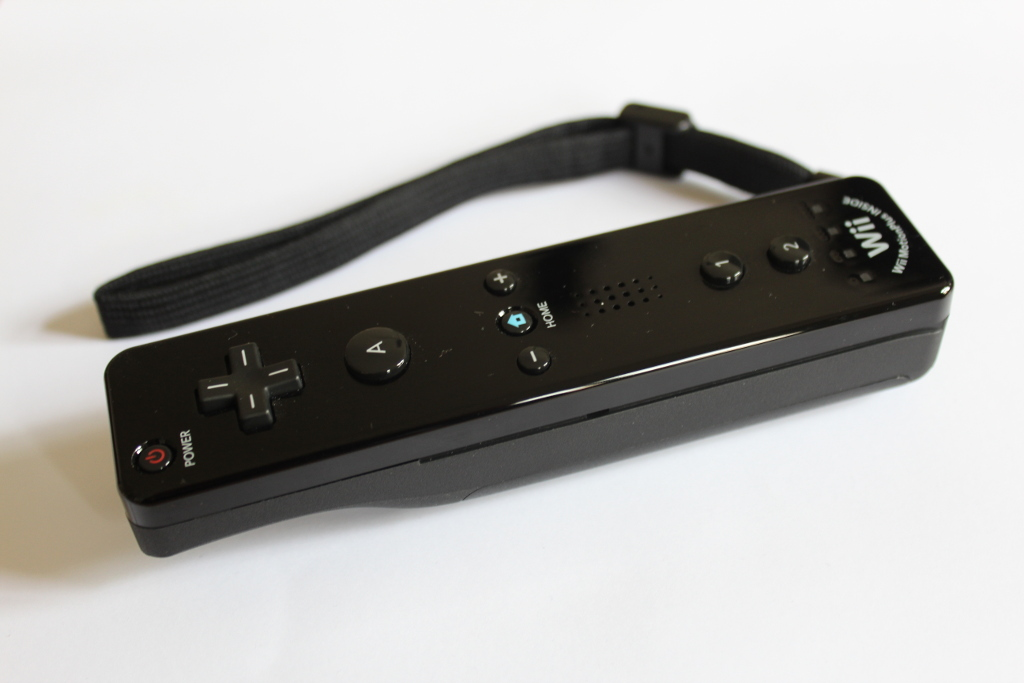
\includegraphics[width=0.5\textwidth]{wii-remote-plus-controller.JPG}
        \end{center}
    \end{itemize}
\end{frame}

\begin{frame}{Evaluation}{Data Recording Instructions}
    \begin{center}
        \resizebox {\textwidth} {!} {
            \begin{tabular}{ccccc}
                \frame{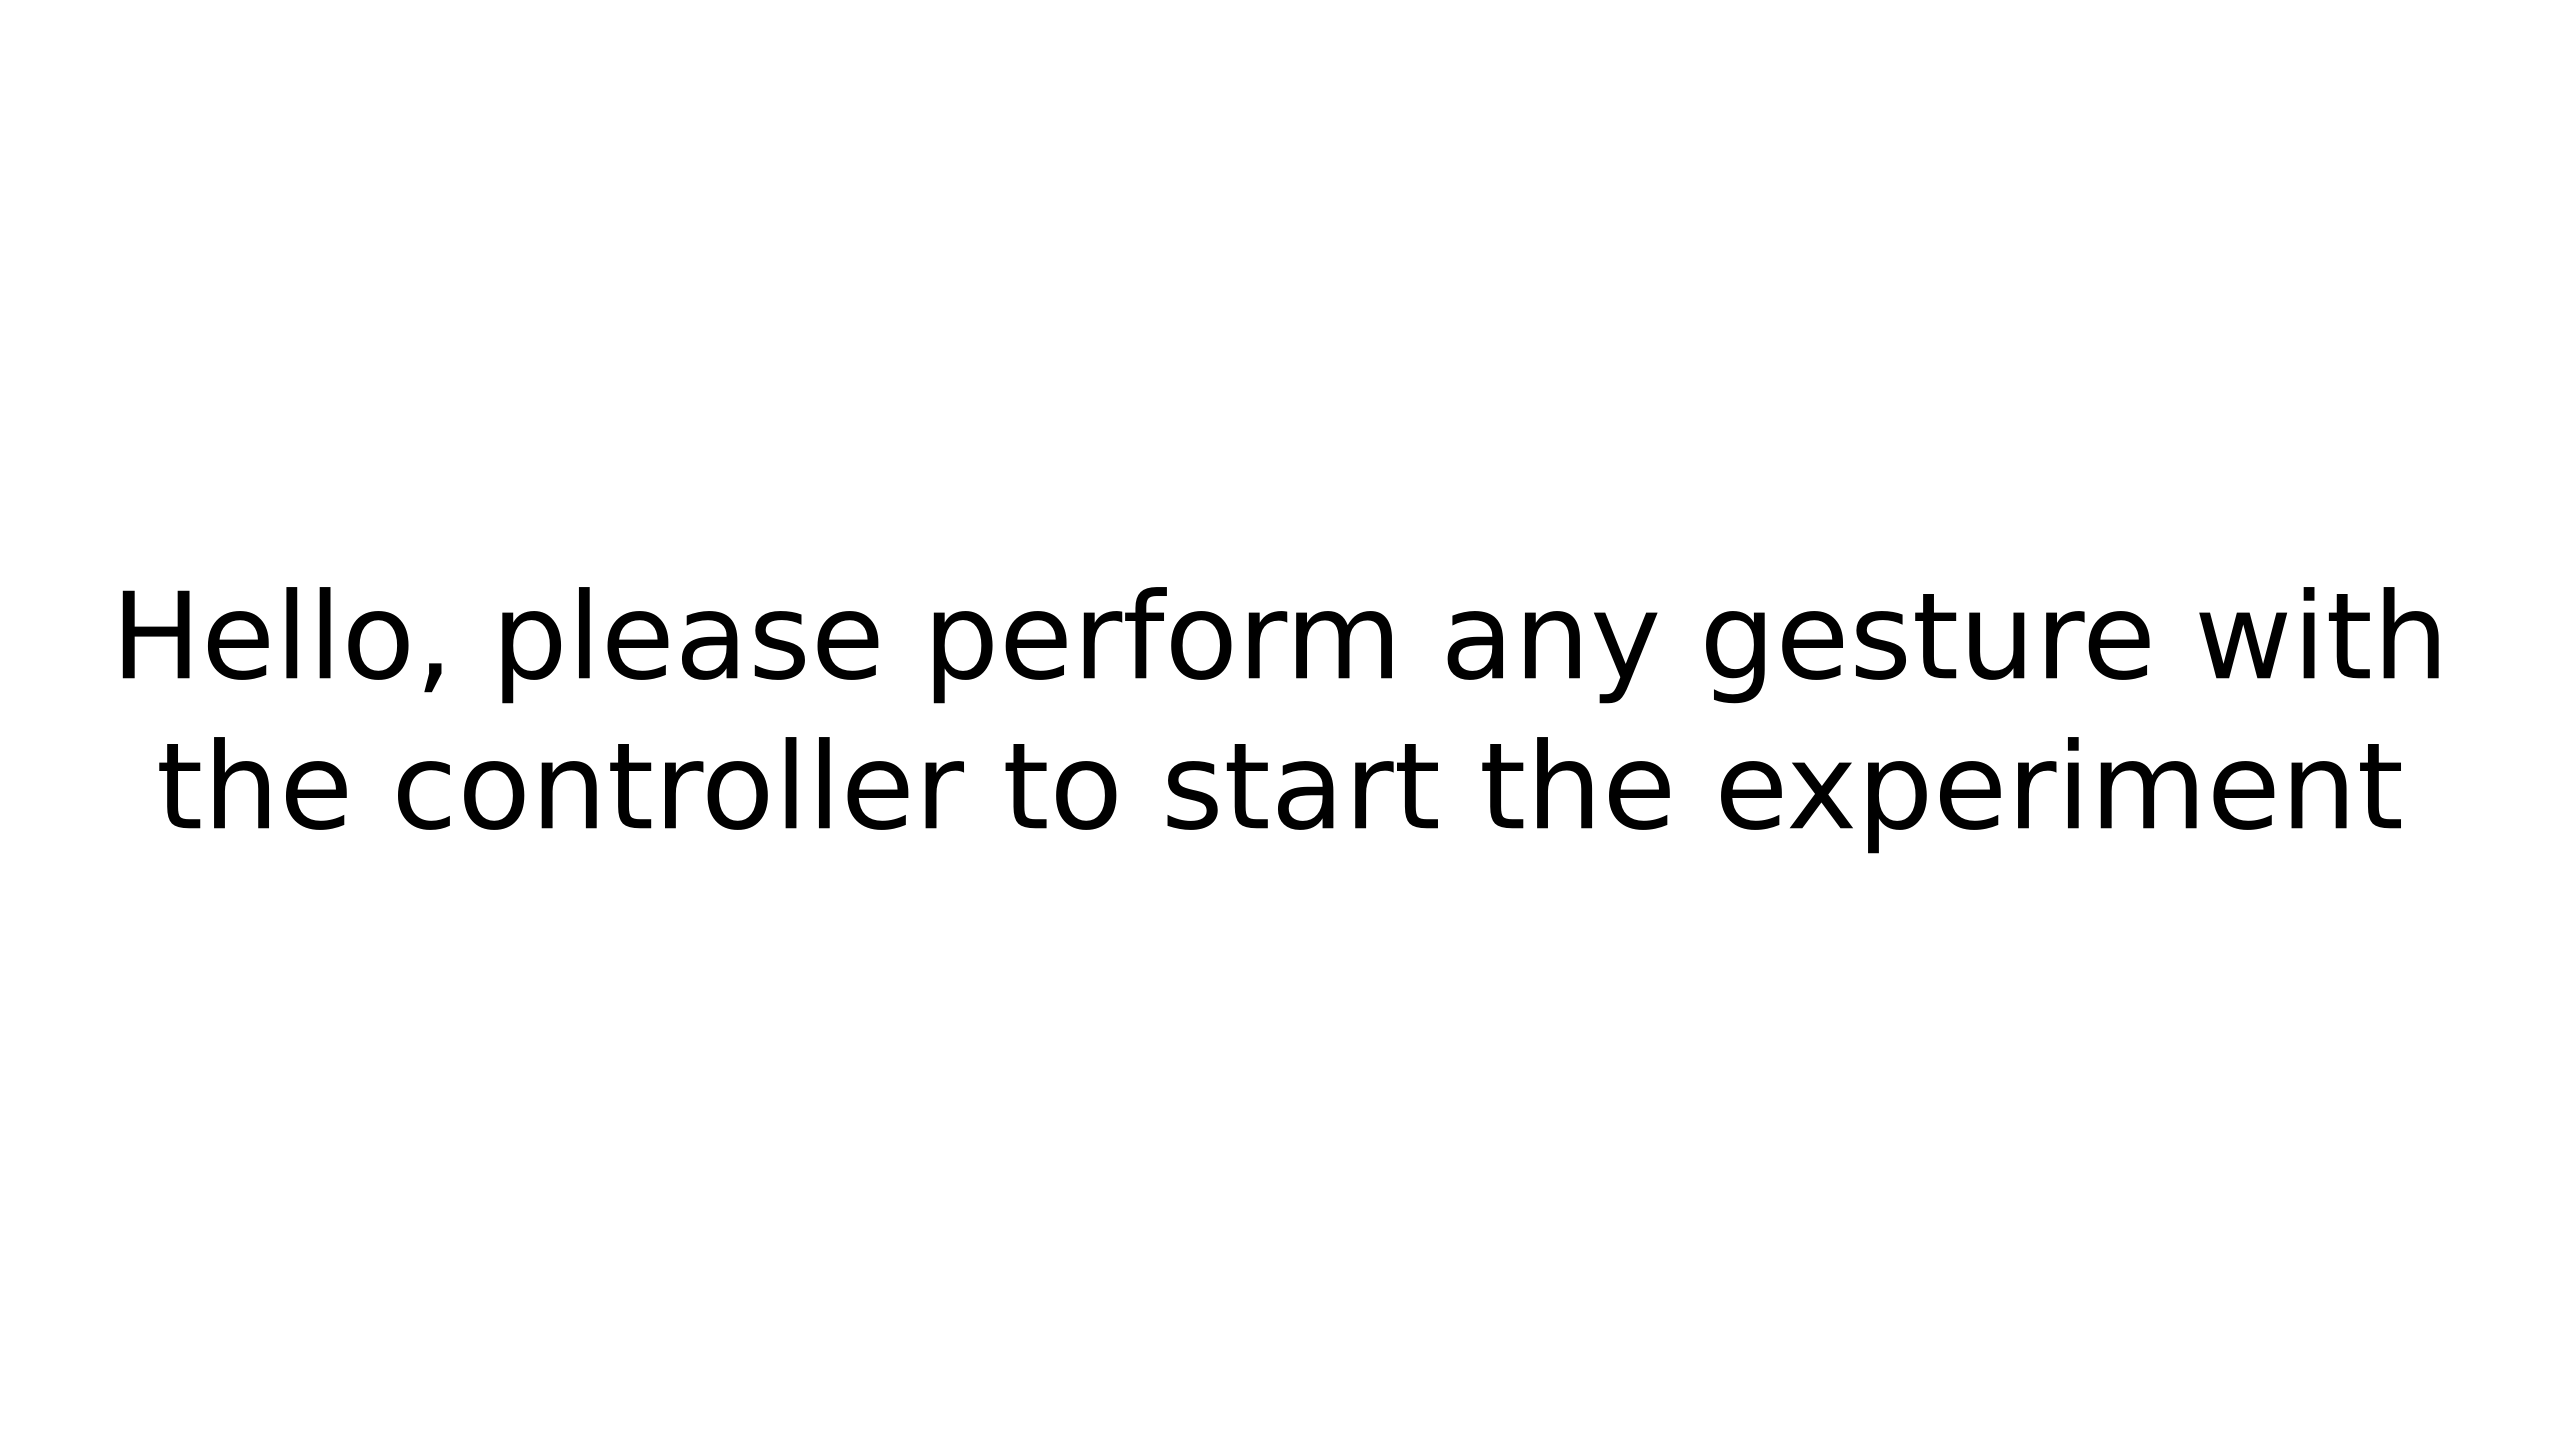
\includegraphics[width=0.25\textwidth]{1.png}} &
                \frame{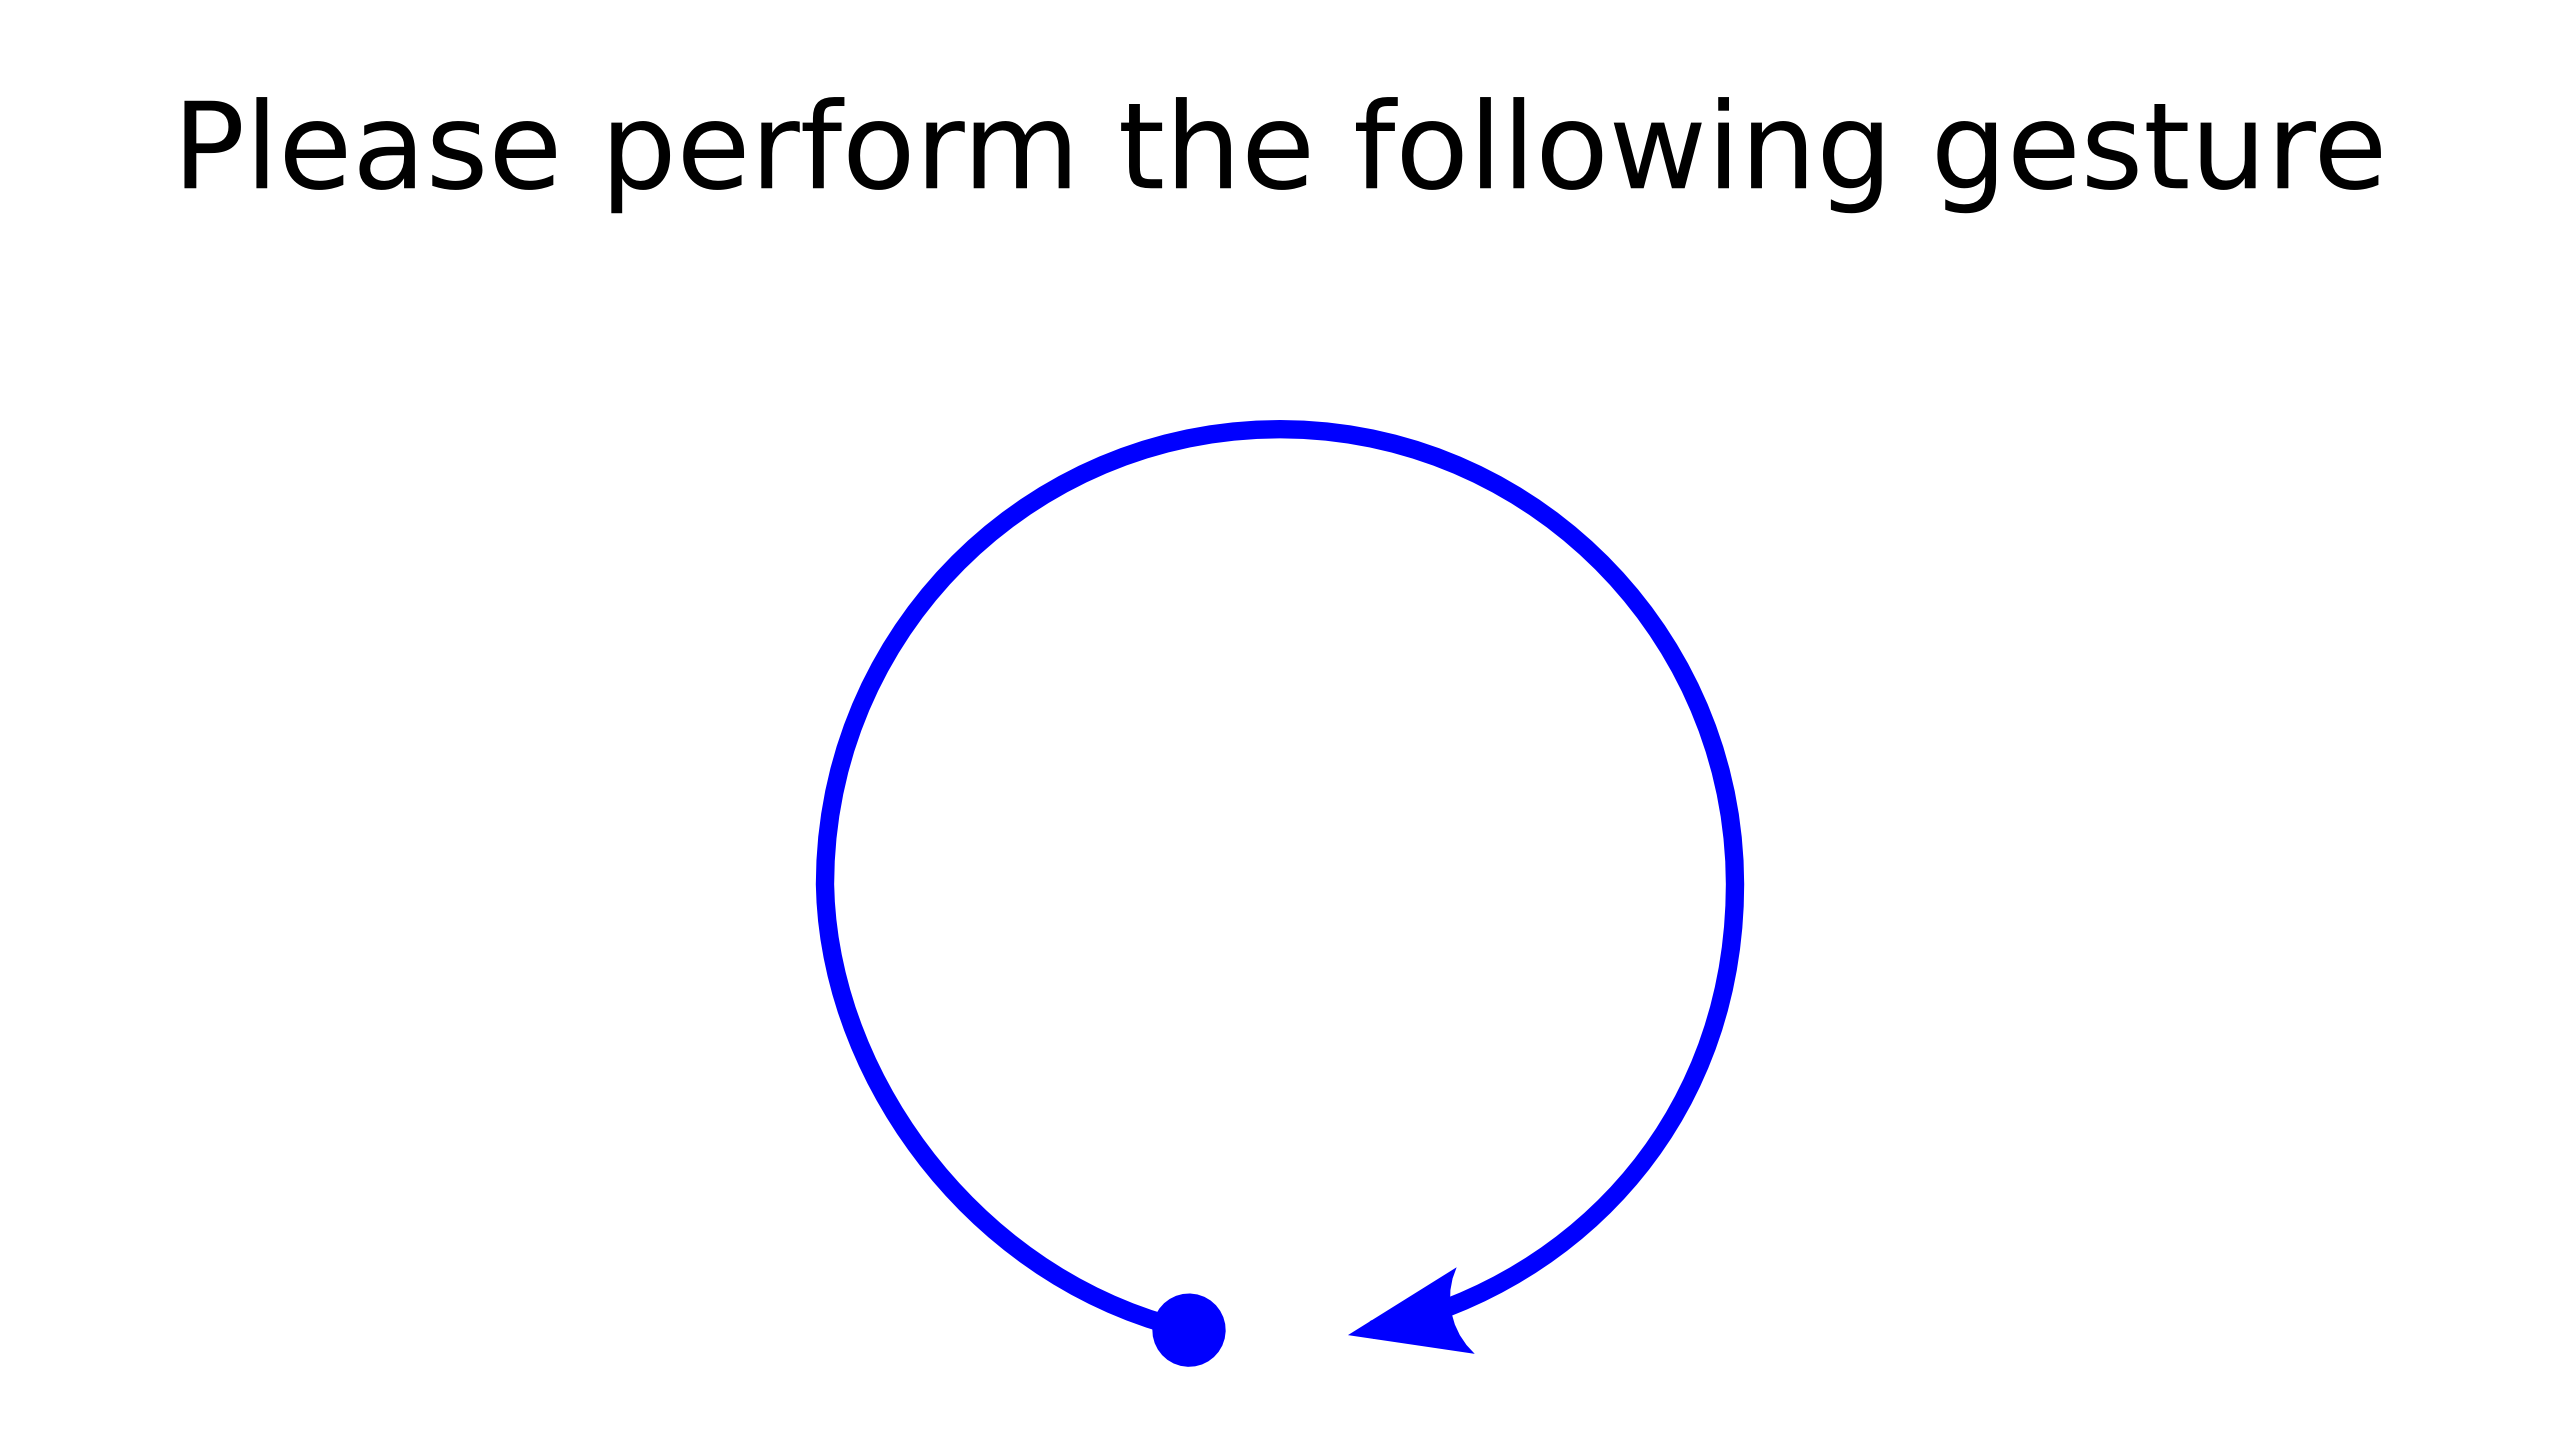
\includegraphics[width=0.25\textwidth]{2.png}} &
                \frame{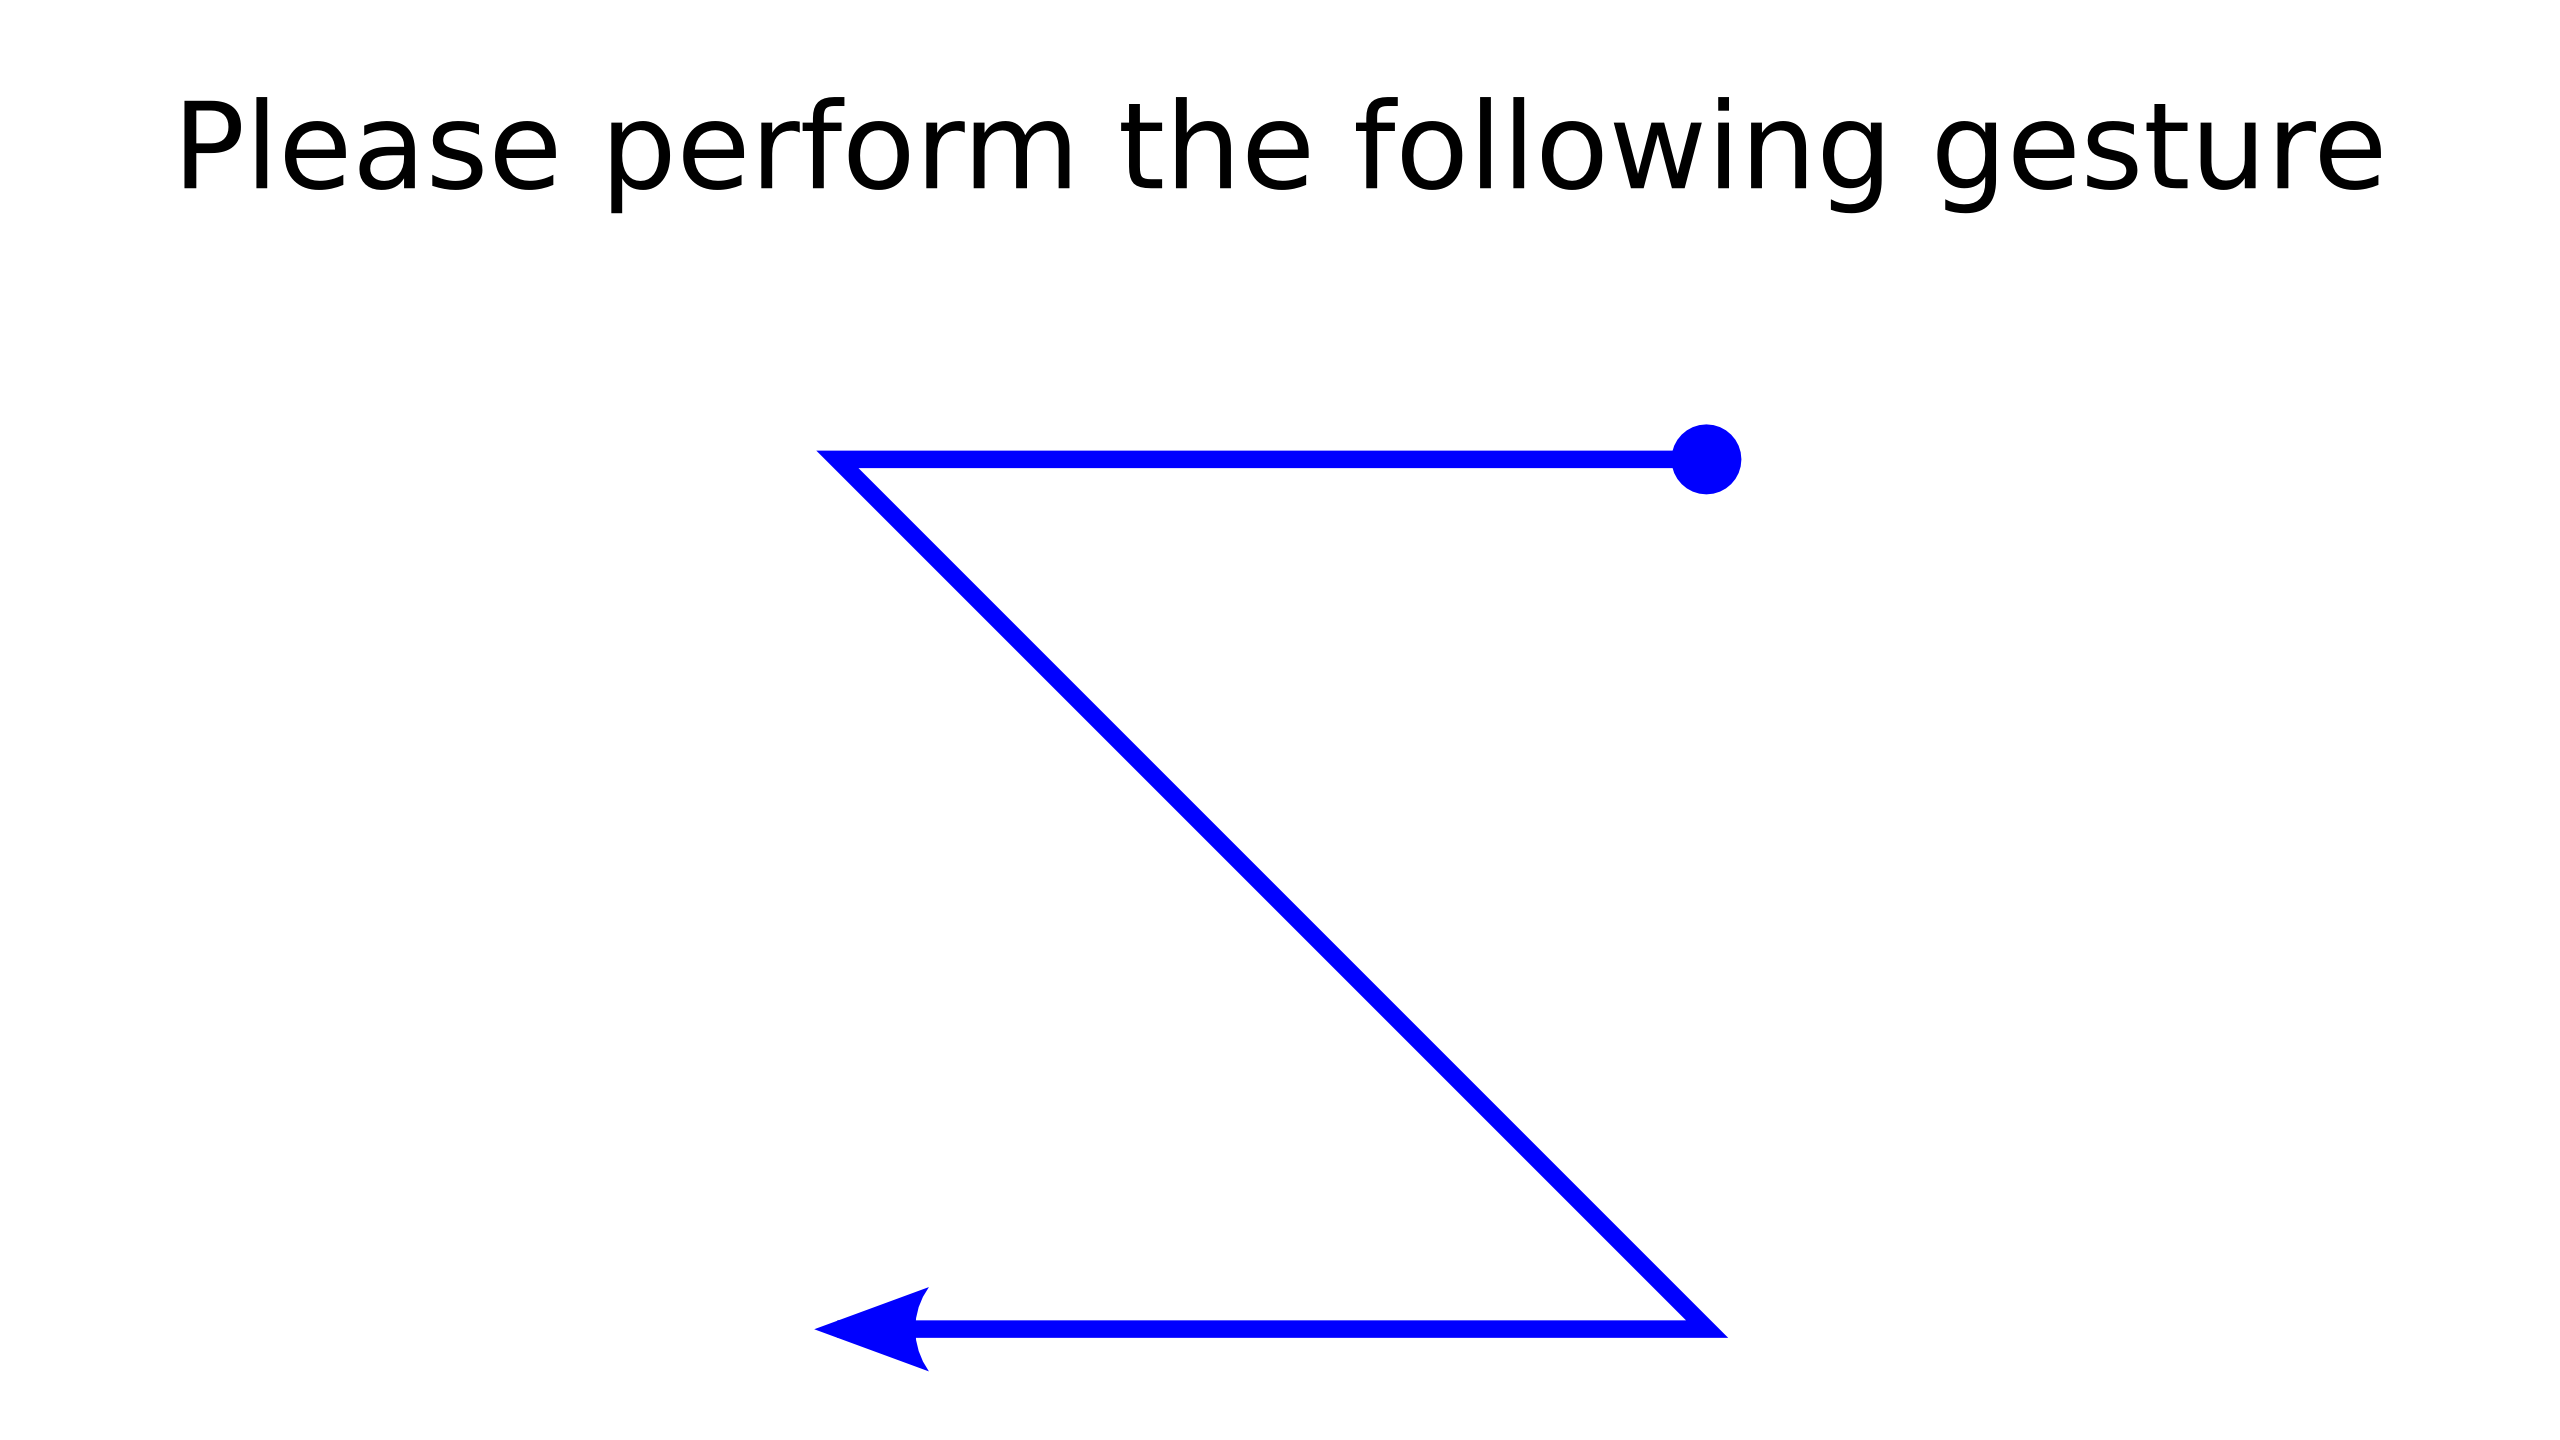
\includegraphics[width=0.25\textwidth]{3.png}} &
                \frame{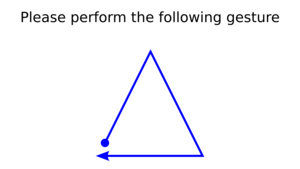
\includegraphics[width=0.25\textwidth]{4.png}} &
                \frame{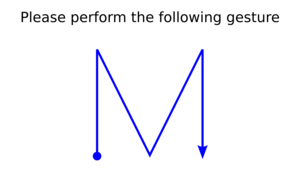
\includegraphics[width=0.25\textwidth]{5.png}} \\
                \frame{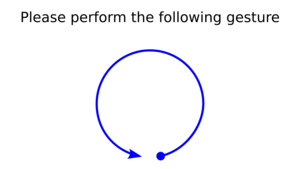
\includegraphics[width=0.25\textwidth]{6.png}} &
                \frame{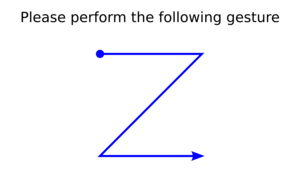
\includegraphics[width=0.25\textwidth]{7.png}} &
                \frame{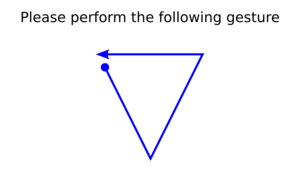
\includegraphics[width=0.25\textwidth]{8.png}} &
                \frame{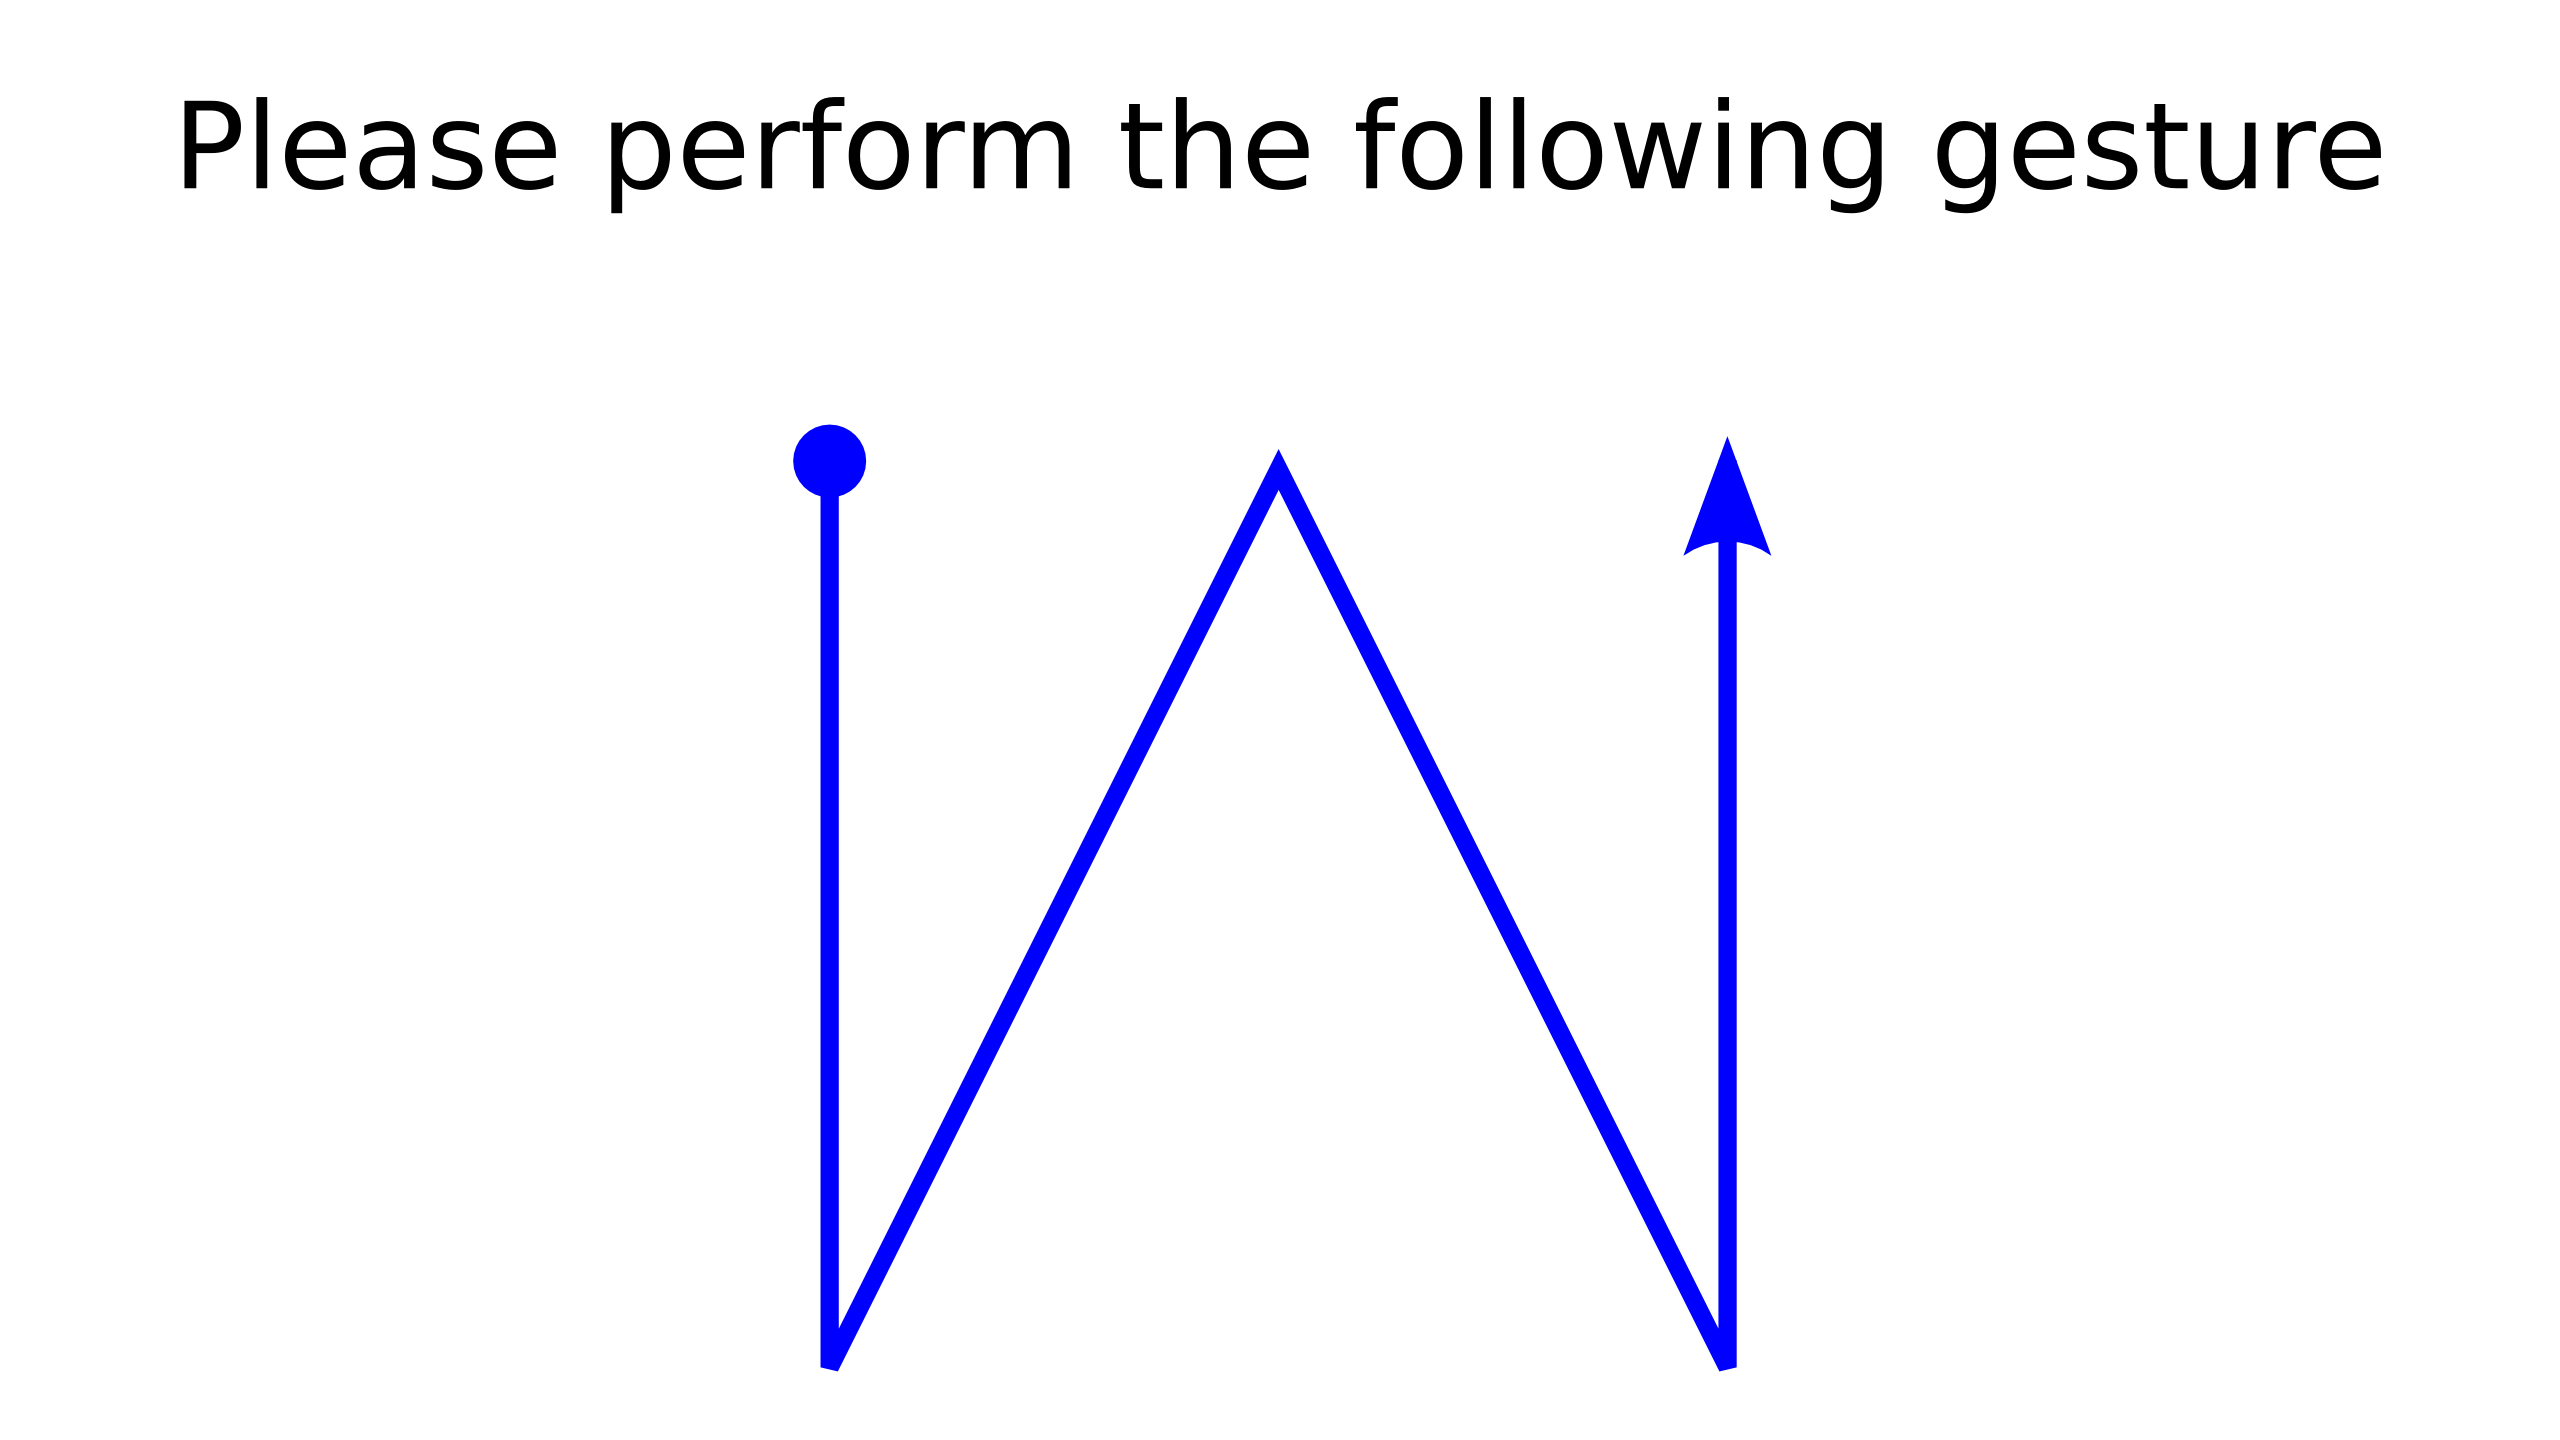
\includegraphics[width=0.25\textwidth]{9.png}} &
                \frame{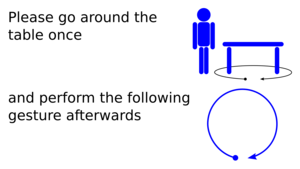
\includegraphics[width=0.25\textwidth]{10.png}} \\
                \frame{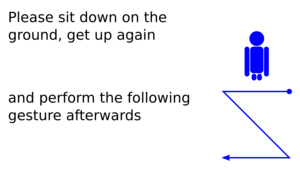
\includegraphics[width=0.25\textwidth]{11.png}} &
                \frame{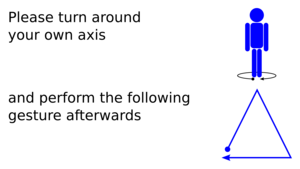
\includegraphics[width=0.25\textwidth]{12.png}} &
                \frame{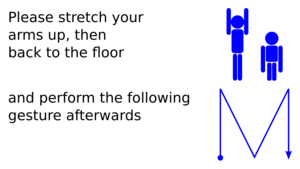
\includegraphics[width=0.25\textwidth]{13.png}} &
                \frame{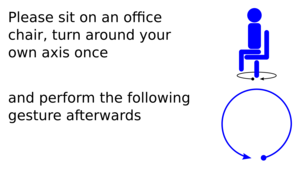
\includegraphics[width=0.25\textwidth]{14.png}} &
                \frame{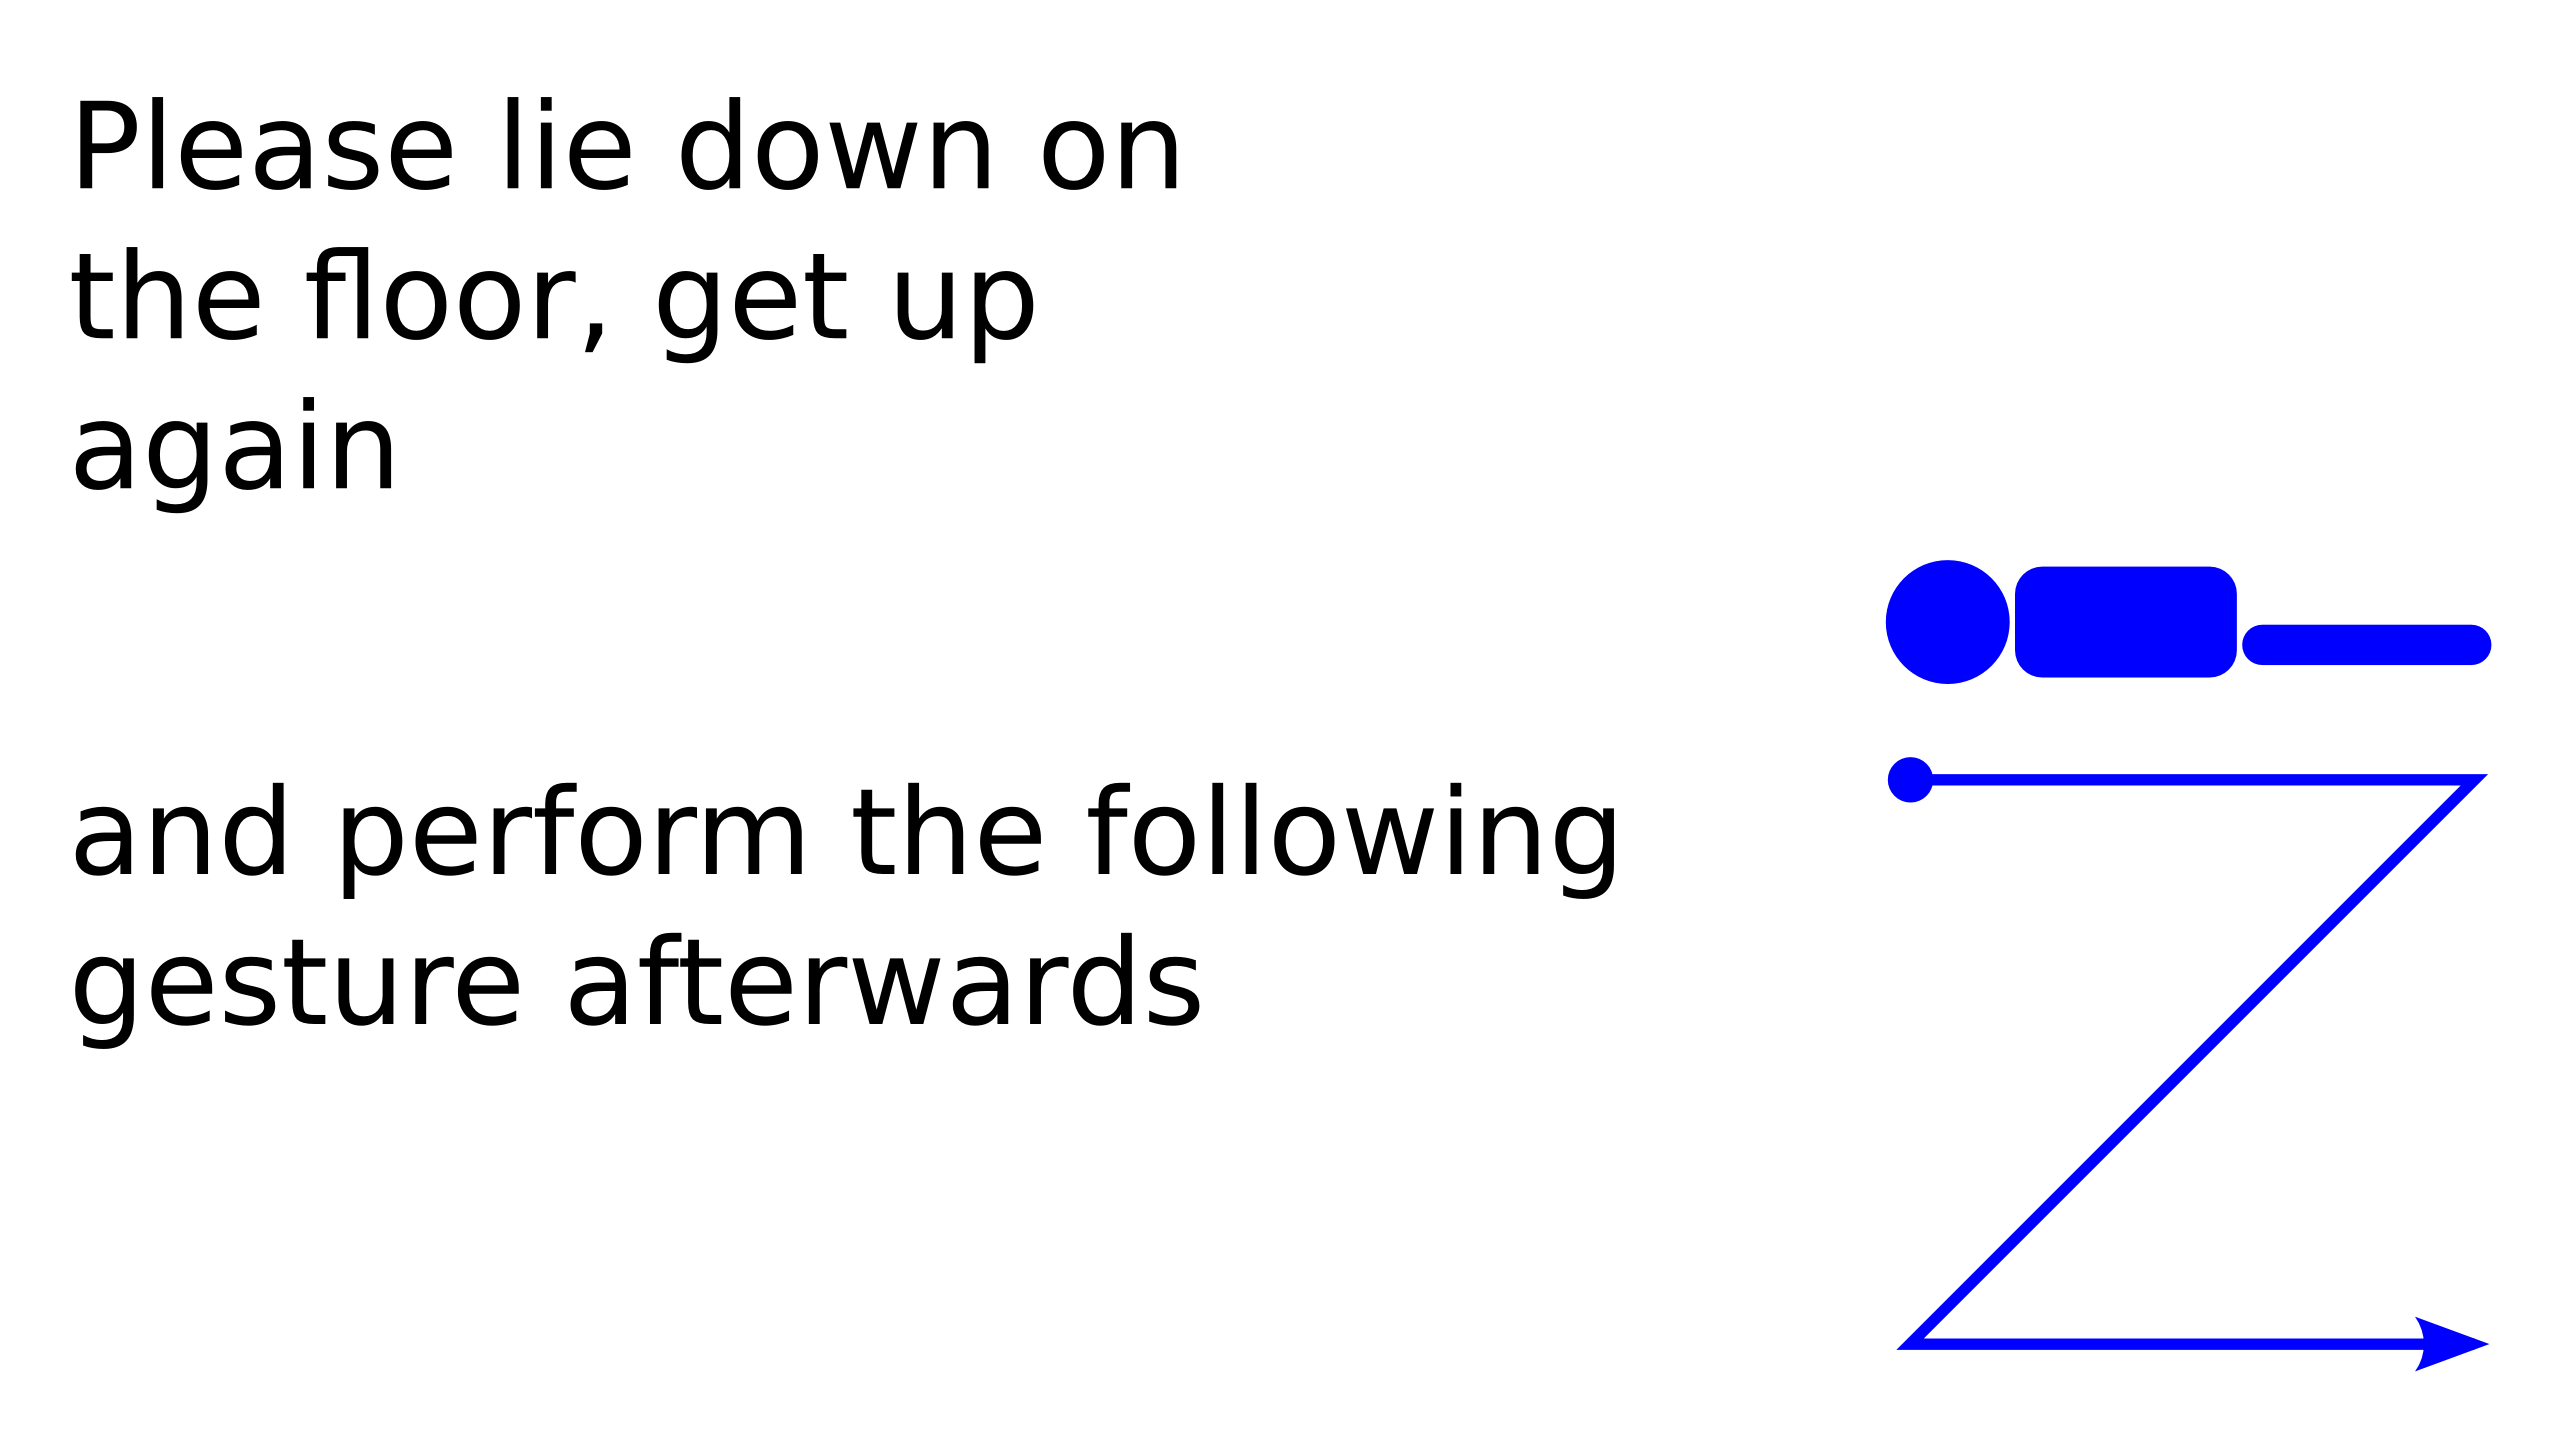
\includegraphics[width=0.25\textwidth]{15.png}} \\
                \frame{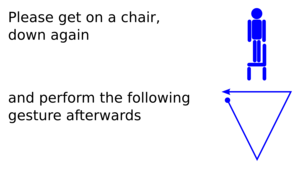
\includegraphics[width=0.25\textwidth]{16.png}} &
                \frame{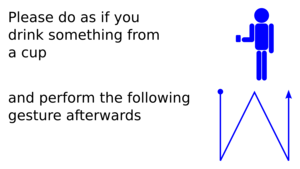
\includegraphics[width=0.25\textwidth]{17.png}} &
                \frame{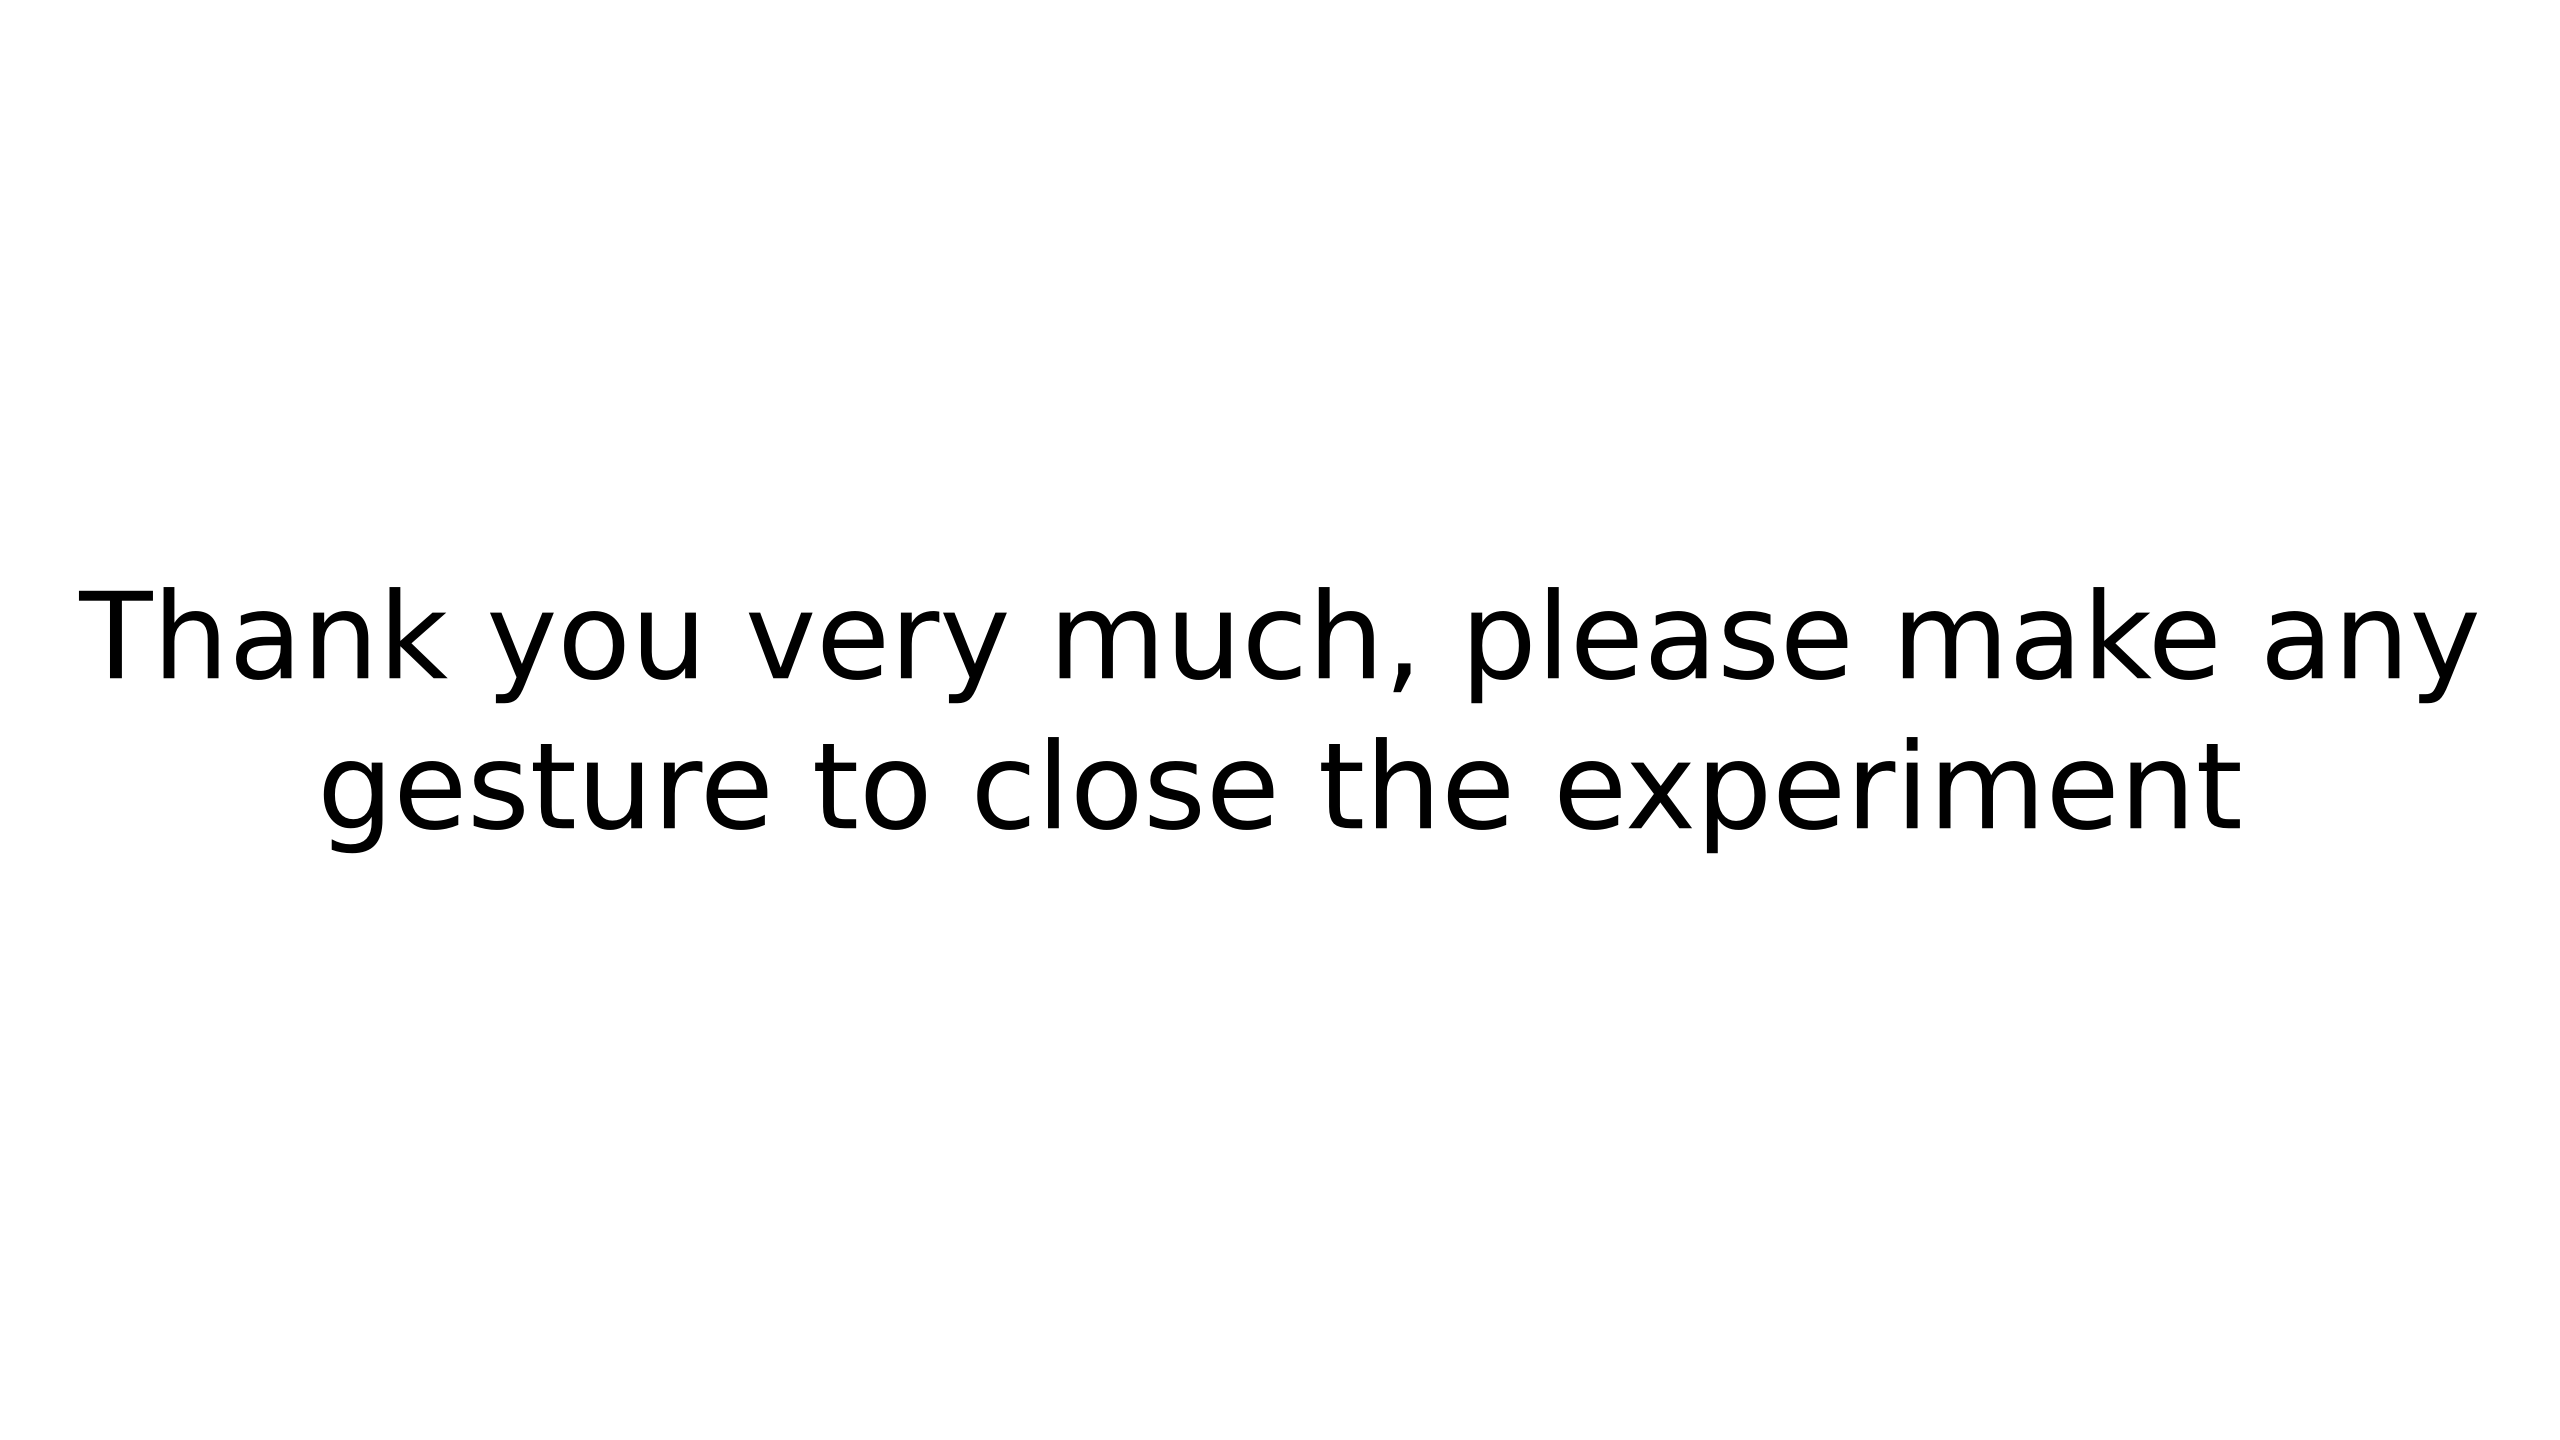
\includegraphics[width=0.25\textwidth]{18.png}} &
                \frame{
\includegraphics[width=0.25\textwidth]{19.png}} \\
            \end{tabular}
        }
    \end{center}
\end{frame}

\begin{frame}{Evaluation}{Recording Example}
    \resizebox {\textwidth} {!} {
        \begin{tikzpicture}
            \begin{axis}[
                xmin=0,
                xmax=3176,
                ymin=-16,
                ymax=16,
                width=10*\axisdefaultwidth,
                height=\axisdefaultheight,
                xticklabels={,,},
                yticklabels={,,}]
                \addplot[blue, mark=none, opacity=0.4] table[x=t, y=x] {../data/fig/record1/timeseries.dat};
                \addplot[red, mark=none, opacity=0.4] table[x=t, y=y] {../data/fig/record1/timeseries.dat};
                \addplot[green, mark=none, opacity=0.4] table[x=t, y=z] {../data/fig/record1/timeseries.dat};
                \addplot+[fill, opacity=0.5, blue, mark=none] coordinates {(38, -16) (89, -16) (89, 16) (38, 16)} --cycle;
                \addplot+[fill, opacity=0.5, blue, mark=none] coordinates {(123, -16) (177, -16) (177, 16) (123, 16)} --cycle;
                \addplot+[fill, opacity=0.5, blue, mark=none] coordinates {(201, -16) (256, -16) (256, 16) (201, 16)} --cycle;
                \addplot+[fill, opacity=0.5, blue, mark=none] coordinates {(282, -16) (355, -16) (355, 16) (282, 16)} --cycle;
                \addplot+[fill, opacity=0.5, blue, mark=none] coordinates {(388, -16) (439, -16) (439, 16) (388, 16)} --cycle;
                \addplot+[fill, opacity=0.5, blue, mark=none] coordinates {(473, -16) (530, -16) (530, 16) (473, 16)} --cycle;
                \addplot+[fill, opacity=0.5, blue, mark=none] coordinates {(568, -16) (624, -16) (624, 16) (568, 16)} --cycle;
                \addplot+[fill, opacity=0.5, blue, mark=none] coordinates {(672, -16) (749, -16) (749, 16) (672, 16)} --cycle;
                \addplot+[fill, opacity=0.5, blue, mark=none] coordinates {(1057, -16) (1106, -16) (1106, 16) (1057, 16)} --cycle;
                \addplot+[fill, opacity=0.5, blue, mark=none] coordinates {(1258, -16) (1313, -16) (1313, 16) (1258, 16)} --cycle;
                \addplot+[fill, opacity=0.5, blue, mark=none] coordinates {(1472, -16) (1527, -16) (1527, 16) (1472, 16)} --cycle;
                \addplot+[fill, opacity=0.5, blue, mark=none] coordinates {(1690, -16) (1772, -16) (1772, 16) (1690, 16)} --cycle;
                \addplot+[fill, opacity=0.5, blue, mark=none] coordinates {(2066, -16) (2116, -16) (2116, 16) (2066, 16)} --cycle;
                \addplot+[fill, opacity=0.5, blue, mark=none] coordinates {(2439, -16) (2497, -16) (2497, 16) (2439, 16)} --cycle;
                \addplot+[fill, opacity=0.5, blue, mark=none] coordinates {(2840, -16) (2895, -16) (2895, 16) (2840, 16)} --cycle;
                \addplot+[fill, opacity=0.5, blue, mark=none] coordinates {(3061, -16) (3137, -16) (3137, 16) (3061, 16)} --cycle;
            \end{axis}
        \end{tikzpicture}
    }
\end{frame}

\begin{frame}{Evaluation}{Data Preparation}
    \begin{itemize}
        \item \textit{Resampling}: data was resampled by means of the moving average technique, using a window size of 50 ms and step size of 30 ms
        \item \textit{Quantization}: converted into time series with integer values between -16 and 16, such as suggested in related work \cite{liu2009uwave}\\
        \begin{center}
            \tiny
            \begin{tabular}{cc}
                \hline
                \textbf{Acceleration data ($a$) in $\frac{dm}{s^2}$} & \textbf{Converted value}\\
                \hline
                $a > 200$ & 16\\
                $100 < a < 200$ & 11 to 15 (five levels linearly)\\
                $0 < a < 100$ & 1 to 10 (ten levels linearly)\\
                $a = 0$ & 0\\
                $-100 < a < 0$ & -1 to - 10 (ten levels linearly)\\
                $-200 < a < -100$ & -11 to - 15 (five levels linearly)\\
                $a < -200$ & -16\\
                \hline
            \end{tabular}
        \end{center}
    \end{itemize}
\end{frame}

\begin{frame}{Evaluation}{Data Preparation Example}
    \begin{center}
        \resizebox {\textwidth} {!} {
            \begin{tabular}{ccc}
                \resizebox {!} {\height} {
                    \begin{tikzpicture}
                        \begin{axis}[
                            xmin=1,
                            xmax=295,
                            xlabel=time,
                            ylabel=acceleration in $\frac{dm}{s^2}$]
                            \addplot[blue, ultra thick, mark=none] table[x=t, y=x] {../data/fig/quantization/raw.dat};
                            \addplot[red, ultra thick, mark=none] table[x=t, y=y] {../data/fig/quantization/raw.dat};
                            \addplot[green, ultra thick, mark=none] table[x=t, y=z] {../data/fig/quantization/raw.dat};
                        \end{axis}
                    \end{tikzpicture}
                } &
                \resizebox {!} {\height} {
                    \begin{tikzpicture}
                        \pgfplotsset{every axis legend/.append style={
                    		at={(0.5,1.03)},
                    		anchor=south}}
                        \begin{axis}[
                            xmin=1,
                            xmax=52,
                            xlabel=time,
                            ylabel=acceleration in $\frac{dm}{s^2}$,
                            legend columns=4]
                            \addplot[blue, ultra thick, mark=none] table[x=t, y=x] {../data/fig/quantization/compressed.dat};
                            \addlegendentry{x-axis}
                            \addplot[red, ultra thick, mark=none] table[x=t, y=y] {../data/fig/quantization/compressed.dat};
                            \addlegendentry{y-axis}
                            \addplot[green, ultra thick, mark=none] table[x=t, y=z] {../data/fig/quantization/compressed.dat};
                            \addlegendentry{z-axis}
                        \end{axis}
                    \end{tikzpicture}
                } &
                \resizebox {!} {\height} {
                    \begin{tikzpicture}
                        \begin{axis}[
                            xmin=1,
                            xmax=52,
                            xlabel=time,
                            ylabel=converted acceleration]
                            \addplot[blue, ultra thick, mark=none] table[x=t, y=x] {../data/fig/quantization/converted.dat};
                            \addplot[red, ultra thick, mark=none] table[x=t, y=y] {../data/fig/quantization/converted.dat};
                            \addplot[green, ultra thick, mark=none] table[x=t, y=z] {../data/fig/quantization/converted.dat};
                        \end{axis}
                    \end{tikzpicture}
                }
            \end{tabular}
        }
    \end{center}
\end{frame}

\begin{frame}{Experiment}{Model parameters}
    \begin{itemize}
        \item \textit{window size}: determines the number of most recent measurements
            \begin{itemize}
                \item min
                \item max
                \item avg
                \item mid
            \end{itemize}
        \item \textit{step size}: defines the gap between consecutive time series windows
            \begin{itemize}
                \item tenth of the window size
            \end{itemize}
        \item \textit{normalization}: normalization prior to pair-wise comparing sliding windows and training gestures
            \begin{itemize}
                \item $\eta$ normalization
                \item $z$ normalization
                \item no normalization
            \end{itemize}
    \end{itemize}
\end{frame}

\begin{frame}{Experiment}{Model Parameters}
    \begin{itemize}
        \item \textit{Sakoe-Chiba band sizes}:
            \begin{itemize}
                \item 34 different between 1 \% to 100 \%
            \end{itemize}
        \item \textit{threshold}: defines the time series distance at which a sliding window and a training gesture are considered to belong to the same class
            \begin{itemize}
                \item HMinD
                \item HAvgD
                \item HMidD
            \end{itemize}
        \item \textit{filter criterion}:
            \begin{itemize}
                \item VAR
                \item LNCE
                \item no filter
            \end{itemize}
    \end{itemize}
\end{frame}

\begin{frame}{Experiment}{Example Result}
    \resizebox {\textwidth} {!} {
        \begin{tikzpicture}
            \begin{axis}[
                xmin=0,
                xmax=2426,
                ymin=-16,
                ymax=16,
                width=10*\axisdefaultwidth,
                height=\axisdefaultheight,
                xticklabels={,,},
                yticklabels={,,}]
                \addplot[blue, mark=none, opacity=0.4] table[x=t, y=x] {../data/fig/experimentee_result2/exp1.dat};
                \addplot[red, mark=none, opacity=0.4] table[x=t, y=y] {../data/fig/experimentee_result2/exp1.dat};
                \addplot[green, mark=none, opacity=0.4] table[x=t, y=z] {../data/fig/experimentee_result2/exp1.dat};
                \addplot+[fill, opacity=0.5, red, mark=none] coordinates {(294, -16) (307, -16) (307, 16) (294, 16)} --cycle;
                \addplot+[fill, opacity=0.5, green, mark=none] coordinates {(307, -16) (357, -16) (357, 16) (307, 16)} --cycle;
                \addplot+[fill, opacity=0.5, red, mark=none] coordinates {(357, -16) (359, -16) (359, 16) (357, 16)} --cycle;
                \addplot+[fill, opacity=0.5, red, mark=none] coordinates {(497, -16) (508, -16) (508, 16) (497, 16)} --cycle;
                \addplot+[fill, opacity=0.5, green, mark=none] coordinates {(508, -16) (562, -16) (562, 16) (508, 16)} --cycle;
                \addplot+[fill, opacity=0.5, blue, mark=none] coordinates {(562, -16) (564, -16) (564, 16) (562, 16)} --cycle;
                \addplot+[fill, opacity=0.5, red, mark=none] coordinates {(712, -16) (722, -16) (722, 16) (712, 16)} --cycle;
                \addplot+[fill, opacity=0.5, green, mark=none] coordinates {(722, -16) (777, -16) (777, 16) (722, 16)} --cycle;
                \addplot+[fill, opacity=0.5, blue, mark=none] coordinates {(777, -16) (778, -16) (778, 16) (777, 16)} --cycle;
                \addplot+[fill, opacity=0.5, blue, mark=none] coordinates {(940, -16) (945, -16) (945, 16) (940, 16)} --cycle;
                \addplot+[fill, opacity=0.5, green, mark=none] coordinates {(945, -16) (1010, -16) (1010, 16) (945, 16)} --cycle;
                \addplot+[fill, opacity=0.5, blue, mark=none] coordinates {(1010, -16) (1023, -16) (1023, 16) (1010, 16)} --cycle;
                \addplot+[fill, opacity=0.5, red, mark=none] coordinates {(1310, -16) (1316, -16) (1316, 16) (1310, 16)} --cycle;
                \addplot+[fill, opacity=0.5, green, mark=none] coordinates {(1316, -16) (1367, -16) (1367, 16) (1316, 16)} --cycle;
                \addplot+[fill, opacity=0.5, red, mark=none] coordinates {(1367, -16) (1375, -16) (1375, 16) (1367, 16)} --cycle;
                \addplot+[fill, opacity=0.5, red, mark=none] coordinates {(1681, -16) (1689, -16) (1689, 16) (1681, 16)} --cycle;
                \addplot+[fill, opacity=0.5, green, mark=none] coordinates {(1689, -16) (1746, -16) (1746, 16) (1689, 16)} --cycle;
                \addplot+[fill, opacity=0.5, blue, mark=none] coordinates {(1746, -16) (1748, -16) (1748, 16) (1746, 16)} --cycle;
                \addplot+[fill, opacity=0.5, red, mark=none] coordinates {(2082, -16) (2090, -16) (2090, 16) (2082, 16)} --cycle;
                \addplot+[fill, opacity=0.5, green, mark=none] coordinates {(2090, -16) (2146, -16) (2146, 16) (2090, 16)} --cycle;
                \addplot+[fill, opacity=0.5, red, mark=none] coordinates {(2146, -16) (2147, -16) (2147, 16) (2146, 16)} --cycle;
                \addplot+[fill, opacity=0.5, blue, mark=none] coordinates {(2311, -16) (2388, -16) (2388, 16) (2311, 16)} --cycle;
                \addplot+[fill, opacity=0.5, red, mark=none] coordinates {(2297, -16) (2362, -16) (2362, 16) (2297, 16)} --cycle;
            \end{axis}
        \end{tikzpicture}
    }
\end{frame}

\begin{frame}{Performance Measures}
        $Precision_{\mu} = {\sum \limits_{i=1}^{l} tp_i}  \bigg/  {\sum \limits_{i=1}^{l} (tp_i + fp_i)}$\\
        $Recall_{\mu} = {\sum \limits_{i=1}^{l} tp_i} \bigg/{\sum \limits_{i=1}^{l} (tp_i + fn_i)}$\\
        $F_{\beta}score_{\mu} = {(\beta^2 + 1)Precision_{\mu} Recall_{\mu}} \bigg/ {\beta^2 Precision_{\mu} + Recall_{\mu}}$\\
\end{frame}

\begin{frame}{Evaluation}{Simulations ranked by $F_{1}score_{\mu}$}
    \begin{center}
        \resizebox {0.5\textwidth} {!} {
            \begin{tikzpicture}[spy using outlines={circle, magnification=6, connect spies}]
                \begin{axis}[
                    xmin=0,
                    xmax=1,
                    ymin=0,
                    ymax=1,
                    width=\axisdefaultwidth,
                    height=\axisdefaultwidth,
                    xlabel=$Precision_{\mu}$,
                    ylabel=$Recall_{\mu}$,
                    samples=100,
                    colorbar horizontal,
                    colormap/viridis high res,
                    title=$F_{1}score_{\mu}$]
                    \addplot[only marks, scatter, scatter src=explicit, mark size=1] table[x=x,y=y,meta=fscore] {../data/fig/result2/result.dat};
                    \addplot[gray, domain=0.051:1] {(0.1 * x) / (2 * x - 0.1)};
                    \addplot[gray, domain=0.11:1] {(0.2 * x) / (2 * x - 0.2)};
                    \addplot[gray, domain=0.16:1] {(0.3 * x) / (2 * x - 0.3)};
                    \addplot[gray, domain=0.21:1] {(0.4 * x) / (2 * x - 0.4)};
                    \addplot[gray, domain=0.26:1] {(0.5 * x) / (2 * x - 0.5)};
                    \addplot[gray, domain=0.31:1] {(0.6 * x) / (2 * x - 0.6)};
                    \addplot[gray, domain=0.36:1] {(0.7 * x) / (2 * x - 0.7)};
                    \addplot[gray, domain=0.41:1] {(0.8 * x) / (2 * x - 0.8)};
                    \addplot[gray, domain=0.46:1] {(0.9 * x) / (2 * x - 0.9)};
                    \coordinate (spypoint) at (axis cs:0.8413867433,0.6578651685);
                    \coordinate (magnifyglass) at (axis cs:0.2,0.8);
                \end{axis}
                \spy [size=2cm] on (spypoint)
                    in node[fill=white] at (magnifyglass);
            \end{tikzpicture}
        }
    \end{center}
\end{frame}

\subsection{Discussion} \label{discussion} \label{instructions_review}
The presented recording instructions in section \ref{data_recording_instructions} combined with the recording software
in section \ref{recording_setup} have been created in front of this bachelor thesis and the experiment was performed
while writing this thesis. Unfortunately do the instructions have some weaknesses that occurred during the experiment or
while evaluating the produced data.

\paragraph{Training Data Quantity} The instructions are containing only 8 instances of training gestures for 8 different
classes. That made the determination of a threshold for a class very difficult. It would have been better to produce at
least two or better three instances of a gesture for every class.

\paragraph{Gesture Illustration Size} It was confusing for some experimentess that the gestures on the slides (j) to (q)
had an other size as the gestures on slide (b) to (i) of figure \ref{fig:slides}. The recording had to be repeated,
cause the experimentess performed the gesture scaled to the illustration size on the slide.

Changing the recording instructions during the bachelor thesis due to the above mentioned weaknesses was no option. It
is assumed that more instances for every class in the training data set would result in a better gesture detection.
However, a bigger training set would also expand the passing filter interval in a more natural way. This would result
in smaller blur factors to expand the passing interval of the filter.

